\begin{abstract}
Widrow and Hoff stored neural-network weights in memistors, three-terminal electrochemical cells, in 1960; lithium-ion,
metal-oxide and protonic ECRAM are their modern descendants. We ask, in simulation, how close such devices come to digital
training when every weight update is made of device pulses and the reads are kept ideal (fp32). We compare plain SGD and three
Tiki-Taka-family algorithms on five device specifications, on MNIST, a CIFAR-10 subset and a byte-level language model, with five
seeds that share initialisation and data order across arms. Against SGD with exact updates at the same learning rate,
\RVAllThreeFpN{} pairings (Li-ECRAM and protonic-inspired, each with chopped TTv2 or AGAD) stay within the pre-set margins on all
three tasks, while plain SGD exceeds them on every published device. Against a separately tuned digital Adam no pairing does: on
the language model the best analog result is \RVLmAdamBestGap\,\% worse in bits per byte. Over a factor of four in width no
arm's gap grows detectably beyond the margin; endpoint equivalence was established for one CIFAR pairing only, and an analysis
paired by seed detects growth for another without resolving its size against the margin. A sensitivity sheet with three seeds establishes only a few one-at-a-time
ranges and shows that an earlier asymmetry limit was mostly lost weight range. Against explicit pulse streams the aggregate
update meets preset point-estimate lines on \RYProbeSurMeetsN{} of \RYProbeN{} probes (bootstrap:
\RYProbeSurAtNinetyFiveN), not where clipping removes nearly all of an
update, and ignores shared-line dependence; in training one label and two close rankings change. A conditional energy projection, borrowing an analog inference chip's read efficiency, gives
\RVenSysMin--\RVenChipMax$\times$ less energy per weight-row than an H100, for cells that pass the margin under ideal reads. This
version repairs the simulator after independent reviews and reports how far each repair moved the original results.
\end{abstract}

\section{Introduction}\label{sec:intro}

Training a neural network on a digital processor moves every weight from memory to arithmetic and back at every update.
In 1960, Widrow and Hoff took a different route: they stored each weight of their adaptive ADALINE neuron in a
\emph{memistor}, an electrochemical cell whose conductance is set by the time integral of a current through a third
terminal~\cite{widrow1960adaline,widrow1960switching,widrow1990}. The weight was read without being disturbed, and it was
adapted in place. The device was macroscopic, the cells were wet, and no multilayer learning rule existed yet, so the line ended
with the Madaline hardware of the early 1960s~\cite{widrow1990}. That machine was a working analog learning system.

Sixty years later, three-terminal electrochemical devices have returned at the nanoscale. Lithium-ion
ECRAM~\cite{tang2018,fuller2017}, CMOS-compatible metal-oxide ECRAM~\cite{kim2019}, protonic programmable
resistors~\cite{onen2022,xu2026} and open-loop programmable arrays~\cite{chen2023} all decouple the read path from the write path,
just as the memistor did. They report hundreds to thousands of conductance levels, nanosecond pulses and femtojoule-scale write
energies. In parallel, algorithms for training on imperfect analog weights have matured: the stochastic pulse-coincidence update
of the resistive processing unit (RPU)~\cite{gokmen2016}, Tiki-Taka~\cite{gokmen2020} and its successors
TTv2~\cite{gokmen2021}, chopped TTv2 and AGAD~\cite{rasch2024}, and residual learning with convergence guarantees~\cite{wu2025}.

That electrochemical weights can train small networks is already established: Chen et al.\ trained in situ on an ECRAM array and
simulated larger networks~\cite{chen2023}, and Rasch et al.\ studied reference correction, retention and device requirements for
the TT family~\cite{rasch2024}. Most recently, Wu et al.~\cite{wu2026scale} simulated ECRAM-calibrated Transformers of up to about
123 million parameters with finite converters and device nonidealities, keeping the weight-gradient path digital. Our
contribution is narrower and specific: \emph{a reproducible, seed-matched simulation comparison} of plain SGD and three
device-tolerant algorithms on a catalog of published (or, where nothing is published, labelled hypothetical) electrochemical
devices, with the weight update done entirely in the devices, on three small tasks; a sensitivity analysis against absolute
accuracy lines; and a \emph{conditional} energy projection. Results are stated against two digital baselines: SGD with exact
updates at the same learning rate, and a separately tuned Adam.

What this paper provides:
\begin{enumerate}
\item \textbf{A simulator with stated limits.} Reads are ideal (fp32); only the update is analog. It reproduces selected
      published outcomes of Gokmen and Haensch 2020 under this simplified read model, and the offset-robustness ordering of
      Rasch et al.\ 2024 (Section~\ref{sec:validation}). After an independent review it was repaired (separate random streams, a
      reset made of pulses, the AIHWKIT device presets mapped one to one) and each repair is tested (Section~\ref{sec:methods},
      Appendix~\ref{app:revision}).
\item \textbf{A seed-matched comparison} of SGD, TTv2, chopped TTv2 and AGAD on five device specifications, three tasks (MNIST, a
      CIFAR-10 subset, a byte-level language model on human-written text) and five seeds, with every arm of a seed sharing its
      initial weights and data order (Section~\ref{sec:main}).
\item \textbf{A width study} with per-arm learning rates and an equivalence test (Section~\ref{sec:scale}).
\item \textbf{A sensitivity sheet} against absolute accuracy lines, with the asymmetry sweep repeated at a fixed symmetry point
      so that asymmetry is not confounded with lost weight range (Section~\ref{sec:spec}).
\item \textbf{A conditional energy projection} for the weight-matrix operations, reported only where the device reaches the
      stated quality (Section~\ref{sec:energy}).
\item \textbf{A proposed roadmap} of device experiments and a proposed, unbuilt bench replication protocol of the 1960
      memistor (Section~\ref{sec:roadmap}, Appendix~\ref{app:bench}).
\end{enumerate}

Every experiment was planned in a committed plan before it ran; the plans are internal, timestamped by the repository, not an
external registry. The original runs and the revision runs are kept apart, and every deviation is recorded
(Section~\ref{sec:availability}). All results are simulations, and every device parameter carries a provenance label
(measured, fitted, claimed, estimated or assumed).

\section{Background and related work}\label{sec:background}

\subsection{The memistor (1960)}
Widrow and Hoff introduced the ADALINE and the least-mean-squares (LMS) rule in 1960~\cite{widrow1960switching}. To store its
weights they built the memistor~\cite{widrow1960adaline}. A pencil-lead (graphite) substrate sits in a copper-sulphate plating
bath. Copper is plated onto it or removed from it by a current through a third electrode, and the conductance between the
lead's two ends is sensed with a small AC signal that does not disturb the state. Widrow, Pierce and Angell described elements
with ``thousands'' of analog levels that spanned roughly 100 to 1 ohm in about ten seconds at a few milliamperes; this description
is reported in secondary sources, see~\cite{mouttet2010}. Mouttet analyses the memistor as a three-terminal memristive system
and summarises Widrow's ideal: a conductance linear in the plating charge, reversible, non-volatile and free of
hysteresis~\cite{mouttet2010}. Widrow and Lehr recount that the Madaline~I machine was built in hardware with memistor weights and used for pattern
recognition research~\cite{widrow1990}.
Write noise, up/down asymmetry, retention and endurance were never reported in a form we could find, so in our catalog these
are estimates (Section~\ref{sec:catalog}). The memistor predates Chua's memristor~\cite{chua1971} and its later physical
identification in titanium-oxide films~\cite{strukov2008}. It is the conceptual ancestor of today's three-terminal synaptic
transistors.

\subsection{Device requirements for training}
Gokmen and Vlasov~\cite{gokmen2016} defined the resistive processing unit (RPU). Updates are stochastic pulse trains whose
coincidences change the conductance by a fixed step (stochastic computing,~\cite{gaines1967}). They derived device
specifications for plain SGD on MNIST at a small error penalty: about a thousand levels, up/down asymmetry of a few percent, and
tolerance to large cycle-to-cycle and device-to-device variation. Agarwal et al.~\cite{agarwal2016} reached similar conclusions;
the requirements were extended to convolutional networks~\cite{gokmen2017cnn}, and reviews cover the device
landscape~\cite{burr2017,ielmini2018,sebastian2020,haensch2019}. Mixed-precision schemes~\cite{nandakumar2020} accumulate the
gradient digitally and program the devices rarely. They relax the device demands but give up the fully parallel in-memory update.

\subsection{Algorithms that tolerate asymmetric devices}
Real devices change their conductance by different amounts up and down, and the step depends on the state (soft bounds). Under
plain SGD this acts as an implicit penalty that pulls weights toward each device's symmetry point~\cite{gokmen2020,wu2025}.
\begin{itemize}
\item \textbf{Tiki-Taka (TTv1)}~\cite{gokmen2020} uses two arrays. The gradient is accumulated on an array $A$, and its columns
      are periodically transferred into the weight array $C$, with $W=\gamma A+C$. Asymmetry then acts as a useful decay on $A$
      instead of a bias on $W$.
\item \textbf{TTv2}~\cite{gokmen2021} inserts a digital buffer $H$ between the two arrays. $H$ low-pass filters the reads of $A$,
      and a pulse is sent to $C$ only when a threshold is crossed. TTv2 still needs every device's symmetry point to be
      subtracted by a reference.
\item \textbf{Chopped TTv2 (c-TTv2)} and \textbf{AGAD}~\cite{rasch2024,rasch2023arxiv} remove this sensitivity. A random sign
      modulates the inputs and the reads (c-TTv2). AGAD additionally replaces the static reference with a digital, on-the-fly
      reference taken from the recent history of $A$.
\item \textbf{Residual learning}~\cite{wu2025} gives convergence guarantees for this family.
\end{itemize}
IBM's open-source AIHWKIT~\cite{rasch2021aihwkit} implements these algorithms with fitted device presets, including the
Li-ECRAM and metal-oxide ECRAM presets whose parameters we use. In the revision these two presets are mapped one to one onto
AIHWKIT's own LinearStepDevice model, with its shifted bounds and slope spread, and checked against AIHWKIT's pulse responses
(Section~\ref{sec:catalog}).

\subsection{Electrochemical three-terminal devices}
\begin{itemize}
\item \textbf{Lithium-ion synaptic transistors and ECRAM.} Fuller et al.~\cite{fuller2017} showed a lithium-ion synaptic
      transistor, followed by an ionic floating-gate array~\cite{fuller2019}. Tang et al.~\cite{tang2018} reported Li-WO$_3$ ECRAM
      with about a thousand symmetric, linear states and nanosecond pulses.
\item \textbf{Metal-oxide ECRAM.} Kim et al.~\cite{kim2019} made it CMOS-compatible.
\item \textbf{Protonic resistors.} Onen et al.~\cite{onen2022} reported nanosecond protonic programmable resistors with a
      phosphosilicate-glass electrolyte. In 2026, Xu et al.~\cite{xu2026} quantified cycle-to-cycle (3\%) and device-to-device
      (21\%) variability of BEOL-compatible protonic ECRAM.
\item \textbf{Open-loop programmable arrays.} Chen et al.~\cite{chen2023} demonstrated a $10\times10$ W/YSZ/WO$_x$ array with
      256 states.
\item \textbf{Organic devices.} Organic electrochemical synapses~\cite{vandeburgt2017} extend the family to low voltages.
\end{itemize}
In-situ training on ECRAM hardware has so far been shown on small arrays, for example a $3\times3$ array by Li et
al.~\cite{li2021ecram} and the $10\times10$ array of~\cite{chen2023}. Other memory technologies have gone further. Phase-change and
resistive arrays have trained or run networks at larger scale~\cite{prezioso2015,ambrogio2018,yao2020,wan2022}, and analog-AI
inference chips with on-chip periphery now report measured efficiencies of about 10~TOPS/W~\cite{ambrogio2023,legallo2023}.

\paragraph{Scaling analog training.} Wu et al.~\cite{wu2026scale} co-designed the weight mapping, the optimizer and the
converters, and simulated ECRAM-calibrated Transformers up to about 123 million parameters with finite converter resolution and
device nonidealities. Their weight-gradient path stays digital, so they do not test the fully in-memory update studied here.
The two studies answer complementary questions: what an analog update saves in computation and data movement, and what it
costs in accuracy and calibration. Our models are far smaller (Section~\ref{sec:discussion}).

\section{Methods}\label{sec:methods}

\subsection{Device model}\label{sec:model}
Each analog weight is one device with a normalised state $u\in[-1,1]$ between its own bounds. Its conductance is
$g=g_{\min}+\tfrac{u+1}{2}(g_{\max}-g_{\min})$, and the weight is read differentially as $w=\alpha\,(g-g_{\mathrm{ref}})$. One
nominal pulse moves $u$ by $k=2/n_{\mathrm{states}}$ at mid-range. With asymmetry $a$ the up and down steps are
$k_\pm=k\,s\,(1\pm a/2)$, where $s$ is a per-device step factor with spread $\sigma_{\mathrm{d2d}}$. With saturation (soft
bounds) the steps depend on the state:
\begin{equation}
\Delta u_+ = k_+\,(1-\gamma_+ u),\qquad \Delta u_- = -k_-\,(1+\gamma_- u).
\end{equation}
The per-device slopes $\gamma_\pm$ have a relative spread $\sigma_\gamma$. A device's symmetry point, where an up and a down
pulse cancel, is $u^*=(k_+-k_-)/(k_+\gamma_++k_-\gamma_-)$. The reference $g_{\mathrm{ref}}$ is set at $g(u^*)$ plus a calibration
error of standard deviation $\sigma_r$, in units of the half-range. A constant-step device has no symmetry point and is
referenced at mid-range.

\begin{itemize}
\item \textbf{Several pulses in one update.} When a device receives $n_+$ up and $n_-$ down pulses in one update, the pulses are
      taken as uniformly interleaved, and $\mathrm{d}u/\mathrm{d}s=A-Bu$ is solved exactly over the batch, with
      $A=k_+n_+-k_-n_-$ and $B=k_+\gamma_+n_++k_-\gamma_-n_-$.
\item \textbf{Write noise.} Cycle-to-cycle noise adds a Gaussian with standard deviation $c_{2c}$ times the local step, growing
      as the square root of the pulse count.
\item \textbf{Drift.} Retention loss relaxes $u$ toward the bare state $u=-1$ with a time constant $\tau$ in training steps.
\item \textbf{Bounds.} The bounds $g_{\min}$, $g_{\max}$ carry a device-to-device spread.
\end{itemize}

\paragraph{The AIHWKIT LinearStepDevice (revision).} The two devices taken from AIHWKIT presets (Li-ECRAM, MO-ECRAM) use
AIHWKIT's own parameterisation instead: the state is the weight itself, with hard bounds $b_{\max}=w_{\max}(1+\sigma_b\xi)$ and
$b_{\min}=w_{\min}(1+\sigma_b\xi)$ around shifted means ($w_{\max}=\RVliWmax$, $w_{\min}=\RVliWmin$ for Li-ECRAM, so that the
symmetry point is at zero), steps $k(1\pm\beta+\sigma_{\mathrm{d2d}}\xi)$, and slopes divided by the mean bounds,
$\Delta w_+=k_+(1-|\gamma_++\sigma_{\gamma+}\xi|\,w/w_{\max})$ and $\Delta w_-=-k_-(1+|\gamma_-+\sigma_{\gamma-}\xi|\,w/|w_{\min}|)$,
with multiplicative write noise. The original version of this paper copied the preset fields into the model above with bounds
$[-1,1]$ and no slope spread; that mapping is kept only for comparison (Appendix~\ref{app:revision}).

Forward and backward passes read the weights ideally, in fp32. Read noise and DAC/ADC quantisation are outside the scope of this
study, which isolates the \emph{update}; the energy projection (Section~\ref{sec:energy}) nevertheless prices finite-precision
reads, so accuracy and energy rest on different read assumptions. Biases, layer norms and the language model's position
table are digital.

\subsection{The update}\label{sec:update}
We use the stochastic pulse-coincidence scheme of~\cite{gokmen2016}. Each sample (row) offers $BL=31$ pulse slots. Input $i$
fires with probability $p_{x,i}\propto|x_i|$ and error $j$ with probability $p_{d,j}\propto|d_j|$, with the scaling split equally
between the two streams (update management). Weight $ij$ therefore receives coincidences with mean
$\eta\,|x_i d_j|/(\alpha k)$. Up and down counts are kept separate, so asymmetry is never cancelled digitally. Within a batch the
counts of all samples are summed and drawn from a Poisson distribution with the requested mean. A mini-batch therefore only
groups pulses; it does not average gradients.

This is a surrogate, not a pulse-by-pulse simulation. The mean is exact only while the largest pre-clamp slot probability is at
most one, i.e.\ $(\eta/\alpha k)\max|x|\max|d|\le BL$; beyond that the probabilities are clipped and part of the update is lost.
The repaired simulator records, per layer, the fraction of updates that clipped and the lost fraction of the requested update
(Section~\ref{sec:main}). Discrete pulses do not commute on a state-dependent device (on a 20-level soft-bounds device one up
then one down pulse from $u=0.4$ ends at \RVorderUpDn, the reverse order at \RVorderDnUp, and the batch solution at \RVorderBatch), and independent
per-cell Poisson draws ignore the correlations of shared row and column pulse streams. A larger variance than the binomial one
is therefore not claimed to be conservative. Section~\ref{sec:fidelity} compares the surrogate with explicit pulse streams on
training cases.

\subsection{Algorithms}\label{sec:algos}
\begin{description}
\item[SGD.] The pulses go directly into the weight devices.
\item[TTv1~\cite{gokmen2020}.] The pulses go into an array $A$, and the forward weight is $C+\gamma A$. Every batch, $n_c$ columns
      $j$ of $A$ are read and added to $C$ by a pulsed outer product, $\lambda A_{:,j}\,e_j^{\top}$. $A$ is never reset.
\item[TTv2 (local variant of~\cite{gokmen2021}).] Each read column is added to a digital buffer,
      $H_{:,j}\mathrel{+}=\lambda A_{:,j}/(\alpha k)$. $C$ receives up to 31 pulses where $|H|\ge1$, and $H$ keeps the remainder.
      Optionally the read column of $A$ is reset after the read. Published TTv2 uses single-pulse transfers, forgets a buffer
      element after it fires and does not reset $A$; we name ours a variant and run the published-style form beside it in the
      diagnostic (Appendix~\ref{app:revision}).
\item[The reset of $A$ (revision).] The original simulator moved the read column of $A$ straight to its symmetry point and
      charged $2BL=62$ pulses it never applied (the \emph{ideal reset}). Applied through the device model, those 62 alternating
      pulses leave \RVresetResidPct\,\% of the displacement on the protonic-inspired device. The repaired \emph{pulse reset} uses the
      transfer's own read: a sign-directed train of $\mathrm{round}(|A_{ij}|/\alpha k)$ pulses toward the read zero, re-read
      and corrected once, at most 62 pulses per weight, every pulse applied through the device dynamics (with its write noise,
      state-dependent step and device spread) and counted. The ideal reset is reported only as a labelled variant.
\item[c-TTv2~\cite{rasch2024}.] Chopper signs $c_j\in\{\pm1\}$ modulate the inputs of the $A$ update ($c\odot x$) and demodulate
      the reads ($c_jA_{:,j}$). Each read column's chopper flips with probability $\rho$.
\item[AGAD~\cite{rasch2024}.] The choppers of c-TTv2, plus a digital leaky average of the reads,
      $p_j\leftarrow(1-\beta)p_j+\beta A_{:,j}$. The read is $z_j=c_j(A_{:,j}-p^{\mathrm{ref}}_j)$, and $p^{\mathrm{ref}}_j$ is
      reset to $p_j$ whenever $c_j$ flips.
\end{description}
In the main experiments every TT-family $A$ array uses a learning rate $1/\lambda$ times larger, so that $\lambda\times$ (the $A$
rate) equals the SGD rate; the TTv1 configuration of the published benchmark (Section~\ref{sec:validation}) is the exception
($\eta=0.01$, $\lambda=0.02$, $A$ rate equal to $\eta$). The settings, including the choice between the pulse reset and no
reset, were chosen once on MNIST validation with a mid-quality device that is not in the catalog (Section~\ref{sec:protocol};
Appendix~\ref{app:selection}). We implemented the algorithms from the papers' text; we did not use the authors' code.

\subsection{Device catalog and provenance}\label{sec:catalog}
Table~\ref{tab:rev_catalog} lists the devices as every revised run uses them. Every field carries a provenance label:
\begin{itemize}
\item MEASURED: reported in the paper;
\item FIT: from the AIHWKIT presets fitted to the published devices~\cite{rasch2021aihwkit};
\item CLAIM: a qualitative statement in the paper, translated by us;
\item ESTIMATE: ours;
\item ASSUMED: for example, the 2\% reference error given to every device.
\end{itemize}
The protonic device of~\cite{onen2022} is mostly estimated: the paper reports a thousand up and a thousand down pulses that are
``nearly linear and symmetric'', but no write-noise or variability statistics, and its finite retention is replaced by no
drift. We therefore call it a \emph{protonic-inspired scenario}; a thousand applied pulses are not a demonstration of a
thousand independently programmable states. The original field copy of the Li-ECRAM and MO-ECRAM
rows is kept, labelled as superseded, in Table~\ref{tab:catalog} (Appendix~\ref{app:original}); the revised runs use the one-to-one AIHWKIT mapping above (bounds $[\RVliWmin, \RVliWmax]$ and $[\RVmoWmin, \RVmoWmax]$,
absolute slope spread \RVliGammaDtod). Widrow's memistor is given two specifications,
one as he described it and one pessimistic, together with a pencil-lead cell built today with modern hobby materials
(Appendix~\ref{app:bench}).

% generated by revision2/analyze_rev2.py from records/revision/CATALOG-REV.json (do not edit)
\begin{table*}[t]\centering\footnotesize\caption{Revised device catalog, the configuration of every revised run (simulator units; provenance per field in records/revision/CATALOG-REV.json). $^*$ AIHWKIT's presets mapped one to one onto its LinearStepDevice (shifted bounds, bound-scaled slopes, device spread 0.05 of the slopes and 0.02 of the asymmetry); the others use the paper's model with bounds $[-1,1]$. Columns: levels $n_{\mathrm{st}}$, asymmetry $a$ (device spread), saturation $\gamma_+/\gamma_-$, bounds, write noise $c_{2c}$, step spread $\sigma_{\mathrm{d2d}}$, reference error $\sigma_r$; no drift. The original field-copy catalog is Table~\ref{tab:catalog} (Appendix~\ref{app:original}).}\label{tab:rev_catalog}
\begin{tabular}{llrllllll}\toprule Device & Label & $n_{\mathrm{st}}$ & $a$ & $\gamma_+/\gamma_-$ & bounds & $c_{2c}$ & $\sigma_{\mathrm{d2d}}$ & $\sigma_r$\\\midrule
Li-ECRAM$^*$ & PUBLISHED-FIT & 1000 & 0 & 0.12/0.51 & [-0.83, 1.17] & 0.3 & 0.1 & 0.02\\
MO-ECRAM$^*$ & PUBLISHED-FIT & 7089 & 0 & 0.42/0.73 & [-0.83, 1.17] & 2 & 0.1 & 0.02\\
Protonic-inspired & PARTLY-PUBLISHED & 1000 & 0.05 & 0.20/0.20 & [-1, 1] & 0.3 & 0.1 & 0.02\\
W/WO$_x$ ECRAM & PUBLISHED-FIT & 256 & 0 & 0.63/0.63 & [-1, 1] & 2.048 & 0.023 & 0.02\\
Memistor (optimistic) & CLAIM+ESTIMATE & 1000 & 0.05 & 0.10/0.10 & [-1, 1] & 0.3 & 0.2 & 0.02\\
\bottomrule\end{tabular}\end{table*}


\subsection{Tasks and baselines}\label{sec:tasks}
\begin{description}
\item[MNIST~\cite{lecun1998}.] A 784--256--128--10 tanh MLP; 10 epochs, batch 128, on 55{,}000 training images. 5{,}000 held-out
      training images form the validation set, and the 10{,}000 test images are the test set.
\item[CIFAR-10 subset~\cite{krizhevsky2009}.] Three $3\times3$ convolutions with $c$, $2c$ and $2c$ channels (base $c=32$),
      computed as crossbar matrix products over unfolded patches, then two fully connected layers. 30 epochs, batch 128, on the
      first 10{,}000 images of training batches 1--2. The next 2{,}000 images are the validation set, and the 10{,}000-image
      test set is the test set.
\item[Character LM.] A byte-level, two-layer transformer~\cite{vaswani2017} of width $d$ (base 128) and context 128, trained on
      8\,MB of enwik8~\cite{mahoney2011}, which is human-written Wikipedia text of 2006. 3{,}000 steps of $32\times128$ bytes.
      Every learned weight matrix uses the device model, including the embedding and the head; the activation-dependent
      attention products and the other operations are digital. Validation is the slice's last 0.5\,MB, held out from
      training in selection runs. Test is a separate 0.5\,MB slice.
\end{description}
The first baseline (``FP-SGD'') is the same network, initialisation, data order and update rule with an exact floating-point
weight update. The second is Adam~\cite{kingma2014} on digital twins with the same initialisation and data order and its own
learning rate selected on validation; in the revision it is reported for all three tasks, beside FP-SGD. The gap is FP accuracy minus device
accuracy for classification, in percentage points. For the LM it is the device's bits per byte relative to FP's, minus one, in
percent.

\subsection{Protocol and statistics}\label{sec:protocol}
Every experiment was pre-registered in a committed plan before it ran (Section~\ref{sec:availability}).
\begin{itemize}
\item \textbf{Hyperparameters} were chosen on validation splits only, with an edge rule: whenever the best value of a grid lies
      at its edge, the next half-decade point is added. The learning rate of every device arm in the main table is the FP
      validation choice. The scale study instead tunes each arm separately.
\item \textbf{Statistics.} The main table uses five seeds per arm. Gaps are paired by seed, and we report the mean and a 95\%
      Student-$t$ interval. A cell PASSES when the whole interval lies below the gap line (2\,pp for classification, 5\% for
      the LM), FAILS when it lies wholly above, and is UNRESOLVED otherwise.
\item \textbf{Multiplicity.} We make no correction for multiplicity. The intervals describe each cell, not the family, and a
      best cell chosen among many is optimistic.
\item \textbf{Random streams (revision).} Each seed defines separate generators for the logical initialisation, the data
      order, each tile's device population and the pulse and noise draws, so the paired gap compares runs that share their
      initial weights and their data.
\item \textbf{Width (revision).} The endpoint contrast $D$ (gap at the widest minus the narrowest width) is tested for
      equivalence (TOST at 5\,\%, margins equal to the gap lines); ``no evidence of growth beyond the margin'' when only the upper
      bound is under the margin; never ``flat''.
\item \textbf{Sensitivity (revision).} Each grid point is labelled against the \emph{absolute} line with 3 seeds paired with
      FP-SGD of the same seed; a threshold is the weakest value that passes with every value toward the best end passing.
\end{itemize}

\subsection{Simulator checks}\label{sec:checks}
The simulator is checked by \nChecks{} checks, and each check is shown to fail on at least one deliberately planted fault
(\nFaults{} faults in all). Examples of what the checks cover:
\begin{itemize}
\item the exact-update arm equals PyTorch SGD;
\item the mean pulse update equals the SGD step;
\item alternating pulses converge to the analytic symmetry point, including with per-device slopes;
\item write noise grows as $\sqrt n$;
\item drift relaxes to the bare state;
\item a static read offset is integrated by TTv2, mostly cancelled by c-TTv2 and nearly fully cancelled by AGAD;
\item TTv1 moves $C$ along $+\lambda A$;
\item the SGD and TTv2 paths are bit-identical to the earlier code that produced our preliminary results.
\end{itemize}
The planted faults include a swapped pulse sign, a dropped chopper demodulation and a never-updated AGAD reference.
Both suites run at the start of every compute session and stop it on any failure (Appendix~\ref{app:checks}). The revision
adds \RVnChecks{} checks of the repairs (matched initialisation and data order across arms, a shared device population across
algorithms, resets that charge exactly the pulses they apply, the AIHWKIT LinearStepDevice recurrence, the clipping statistics,
the published-style buffer, the re-centred symmetry point, and a bit-exact replay of the original simulator), each shown to
fail on the old behaviour or a planted fault (Appendix~\ref{app:revision}). These checks test the implementation; they do not
validate the physical model.

\section{Results}\label{sec:results}
\subsection{Simulator validation}\label{sec:validation}
\paragraph{Gokmen and Haensch 2020.} We map their RPU-baseline device onto our model:
\begin{itemize}
\item step $10^{-3}$ at $w=0$;
\item mean saturation slope $1.66$ with a 25\% per-device spread;
\item 30\% step spread and 30\% cycle-to-cycle noise;
\item a symmetry point at $w=0$ for every device.
\end{itemize}
We train their 784--256--128--10 sigmoid network on MNIST for 50 epochs at their learning rate of 0.01. The results are in
Table~\ref{tab:e1} and Fig.~\ref{fig:validation}a.
\begin{itemize}
\item FP reaches \REOneFpErr\% test error, against their 2.0\%.
\item SGD on the device reaches \REOneSgdErr\% [\REOneSgdLo, \REOneSgdHi], against ``about 15\%''.
\item Tiki-Taka reaches \REOneTtvOneErr\% [\REOneTtvOneLo, \REOneTtvOneHi], against ``close to 2\%''.
\end{itemize}
By our pre-registered criteria the agreement is \textbf{\REOneVerdict}: this is agreement with selected published outcomes
under a simplified read model, not a full quantitative validation. Matching an endpoint under different sources of error cannot
rule out compensating differences, and the batch-64 result below shows how sensitive the SGD arm is to the protocol. These
validation runs used the original simulator (TTv1 has no reset, so the reset repair does not touch them). The known
differences are listed in Section~\ref{sec:limits}:
\begin{itemize}
\item we use mini-batches of 16, not 1;
\item we do not model read noise, ADC/DAC quantisation or analog biases.
\end{itemize}
At batch 64 the FP and TTv1 results barely move, but SGD on the device degrades further. Summing more samples' pulses before the
weight changes hurts a strongly asymmetric device, which is another reason to use batch 16 as the closer match to their batch 1.

\paragraph{Rasch et al.\ 2024, qualitatively.} We use a 20-state soft-bounds device with an uncorrected reference offset of
$\sigma_r=0.5$ (Table~\ref{tab:e1b}, Fig.~\ref{fig:validation}b).
\begin{itemize}
\item TTv2's test error rises from \REOnebTtvTwoSrZero\% to \REOnebTtvTwoSrFive\%.
\item c-TTv2 rises less, from \REOnebCttvTwoSrZero\% to \REOnebCttvTwoSrFive\%.
\item AGAD reads \REOnebAgadSrZero\% versus \REOnebAgadSrFive\% (no change detected with two seeds).
\end{itemize}
This is the published ordering; our pre-registered check reads \textbf{\REOnebVerdict}. It rests on two seeds per condition
and an ordering, so it does not establish that our c-TTv2 and AGAD are equivalent to the published implementations, and the
absence of a detected change does not show that AGAD is unaffected. In our implementation AGAD starts from a higher error at
zero offset on this very coarse device.

\paragraph{The device presets against AIHWKIT itself (revision).} On a rented machine (never on our desk) we installed AIHWKIT
\RVaihwVersion{} from PyPI and drove its EcRamPresetDevice and EcRamMOPresetDevice through long up, down and alternating pulse
schedules (500 devices each, with and without cycle-to-cycle noise), using its own plotting utilities. Our AIHWKIT-mode tile,
driven through the same schedules, \RVaihwVerdict{} (largest mean difference \RVaihwLiMaxDiff{} for Li-ECRAM and
\RVaihwMoMaxDiff{} for MO-ECRAM, in weight units; the pre-registered tolerance is $\max(4\,\mathrm{SE},2\,\Delta w_{\min})$ at every
stored pulse). The original field-copy mapping differs by up to \RVaihwLiOldMaxDiff{} for Li-ECRAM, mostly at the bounds
(Appendix~\ref{app:revision}).

% generated by analyze.py (do not edit)
\begin{table}[t]\centering\small\caption{Validation against Gokmen and Haensch 2020 (FCN 784-256-128-10, MNIST, 50 epochs): test error in \%, our mean and 95\% interval over 3 seeds at batch 16, and one seed at batch 64.}\label{tab:e1}
\fitbox{\begin{tabular}{lccc}\toprule
Arm & Published~\cite{gokmen2020} & Ours (batch 16) & Ours (batch 64)\\\midrule
FP (exact update) & 2.0 & 1.78 [1.75, 1.81] & 1.79 (n=1)\\
SGD on the RPU-baseline device & about 15 & 14.47 [12.68, 16.26] & 24.32 (n=1)\\
Tiki-Taka (TTv1) & close to 2 & 2.26 [2.13, 2.39] & 2.07 (n=1)\\
TTv2 (ours, 16 columns per batch) & -- & 2.59 [2.42, 2.75] & not run\\
\bottomrule\end{tabular}}\end{table}

% generated by analyze.py (do not edit)
\begin{table}[t]\centering\small\caption{Qualitative check of Rasch et al.\ 2024 (Fig.~5): a 20-state soft-bounds device with an uncorrected reference offset $\sigma_r$; test error in \% (mean and 95 \% $t$ interval, $n=2$; 10 epochs). FP: 2.69 [0.47, 4.92].}\label{tab:e1b}
\fitbox{\begin{tabular}{lccc}\toprule Offset & TTv2 & c-TTv2 & AGAD\\\midrule
$\sigma_r=0$ & 4.12 [2.79, 5.46] & 4.29 [3.91, 4.67] & 8.47 [7.58, 9.36]\\
$\sigma_r=0.5$ & 24.27 [18.23, 30.30] & 13.02 [10.99, 15.05] & 7.88 [3.49, 12.26]\\
\bottomrule\end{tabular}}\end{table}

\begin{figure}[t]\centering
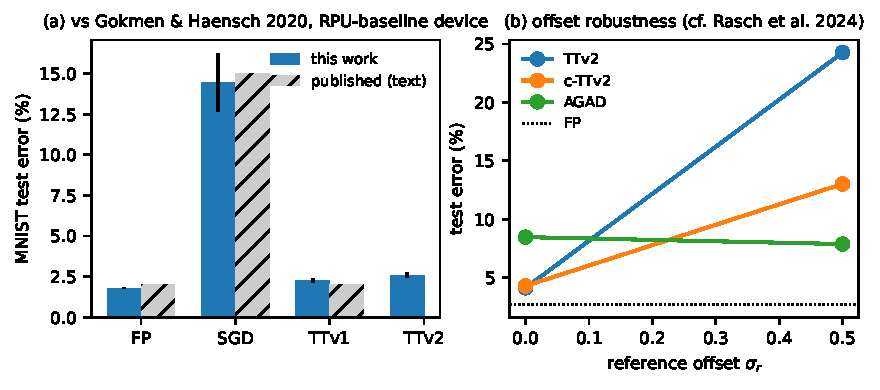
\includegraphics[width=\linewidth]{figs/fig_validation}
\caption{Simulator validation. (a) Test error of our simulator (mean and 95\% interval, 3 seeds) against the values stated in
the text of Gokmen and Haensch 2020 for their FCN on MNIST with the RPU-baseline device. (b) Robustness to an uncorrected
reference offset on a 20-state device (2 seeds), the qualitative trend of Rasch et al.\ 2024, Fig.~5.}\label{fig:validation}
\end{figure}

\subsection{Main comparison on the repaired simulator}\label{sec:main}
Tables~\ref{tab:rev_vs_fp} and~\ref{tab:rev_vs_adam} give the gap of every device--algorithm pairing over five seeds, against
FP-SGD (the same network, learning rate, initialisation and data order with an exact update) and against digital Adam at its
own selected learning rate. Every arm of a seed now shares its initial weights and its data order (checked by hash in every
record). The FP-SGD learning rate is reused for every device arm: this is a restricted question (what happens when the FP-SGD
rate is reused), not a fair-tuning comparison of the algorithms; Section~\ref{sec:scale} tunes each arm separately.

\paragraph{Against FP-SGD.}
\begin{itemize}
\item \textbf{Plain SGD exceeded the line} in \RVSgdPubFail{} of the \RVSgdPubN{} cells of the four published devices, at the
      FP-selected learning rate.
\item \textbf{All three tasks:} \RVAllThreeFpN{} pairings pass on every task: \RVAllThreeFpList. No TTv2 pairing does: with the
      pulse reset, TTv2 fails on CIFAR on every published device.
\item \textbf{Per task,} \RVMnistFpPassN, \RVCifarFpPassN{} and \RVLmFpPassN{} of the \RVMnistFpCellN{} device cells pass on
      MNIST, CIFAR and the LM. W/YSZ/WO$_x$ fails on CIFAR and the LM with every algorithm, and MO-ECRAM fails on the LM.
\item \textbf{Best cells:} \RVMnistFpBestCell{} on MNIST (\RVMnistFpBestGap\,pp), \RVCifarFpBestCell{} on CIFAR
      (\RVCifarFpBestGap\,pp) and \RVLmFpBestCell{} on the LM (\RVLmFpBestGap\,\%). A negative gap whose interval includes zero
      is not evidence of superiority; and because these are the best of many cells, they are optimistic.
\end{itemize}

\paragraph{Against Adam.} Digital Adam is the stronger baseline. On the LM FP-SGD is \RVLmFpSgdVsAdamPct\,\% worse in bits per
byte than Adam, and \textbf{no analog cell comes within the 5\,\% line of Adam}: the best, \RVLmAdamBestCell, is
\RVLmAdamBestGap\,\% worse (\RVLmAdamPassN{} of \RVLmAdamCellN{} cells pass). On MNIST and CIFAR, where Adam and FP-SGD are
close, \RVMnistAdamPassN{} and \RVCifarAdamPassN{} cells pass against Adam. No pairing passes all three tasks against Adam
(\RVAllThreeAdamN). The analog results are therefore close to the FP-SGD comparator on these tasks, not to the best digital
training in this study.

\paragraph{The margins.} The lines are practical non-inferiority margins, not equivalence: on MNIST a 2\,pp loss from
\RVMnistFp\,\% roughly doubles the error rate. UNRESOLVED means insufficient evidence against the margin, never adequate
performance. The mean digital baselines are \RVMnistFp\,\% and \RVMnistAdamMetric\,\% on MNIST, \RVCifarFp\,\% and
\RVCifarAdamMetric\,\% on CIFAR, and \RVLmFp{} and \RVLmAdamMetric{} bits per byte on the LM (FP-SGD and Adam). The FP-SGD seed standard deviation is \RVCifarFpSd\,pp on CIFAR and \RVLmFpSd{} bits per byte on the LM.

\paragraph{What the update loses.} Two properties of the repaired simulator matter for reading these results.
\begin{itemize}
\item \textbf{Clipping.} The TT family drives its $A$ arrays at ten times the SGD rate, which exceeds the $BL=31$ pulse budget
      in the largest layers: the mean lost fraction of the requested $A$ update reaches \RVLostCifarTtLayerMeanMaxPct\,\% in the
      CIFAR output layer and \RVLostLmTtLayerMeanMaxPct\,\% in the LM embedding (plain SGD at most \RVLostLmSgdLayerMeanMaxPct\,\%
      in any layer's mean). These are means over the device runs of one layer; the worst single layer record loses
      \RVLostMaxPct\,\% (\RVLostWorstDev{} \RVLostWorstAlg, \RVLostWorstTask{} output layer). The logged fraction is the
      discarded unsigned expected pulse mass, not the norm of the lost signed gradient after cancellation. Clipping the line
      probabilities at one is the update-management policy chosen here (pulse length and update management are configurable
      choices~\cite{rasch2021aihwkit}), not a property of the devices; it caps the effective $A$ rate in those layers, and the
      aggregate update itself is an approximation (Section~\ref{sec:fidelity}).
\item \textbf{Reset residual.} With at most 62 pulses per weight, the pulse reset leaves a residual on the read $A$
      columns. Averaged with every layer and run weighted equally (a macro-average of the per-layer means), it is
      \RVResetResidMean{} nominal steps; pooled over all reset events it is \RVResetResidPooled{} (Li-ECRAM
      \RVResetResidPooledEcramLiTangTwoZeroOneEight, protonic-inspired \RVResetResidPooledProtonicOnenTwoZeroTwoTwo, MO-ECRAM
      \RVResetResidPooledEcramMoKimTwoZeroOneNine); the largest layer mean is \RVResetResidMax{} (MO-ECRAM). Reset pulses are
      \RVResetShareMean\,\% of all pulses as the mean of the per-run fractions, and \RVResetSharePooled\,\% pooled (all reset
      pulses over all pulses). The macro-averages say what a typical layer and run see; the pooled numbers what the arrays
      receive in total.
\end{itemize}

\paragraph{Ideal-device reference.} The same algorithms on an ideal device (symmetric, constant step, 1000 levels, no noise, no
spread, exact reference) are the rows ``Ideal 1000-level'' of the tables (deviation R2). On MNIST every algorithm passes on it.
On CIFAR and the LM none does: plain SGD loses \RVCifarIdealOneZeroZeroZeroSgdVsFpGap\,pp and
\RVLmIdealOneZeroZeroZeroSgdVsFpGap\,\% (stochastic pulse updates on a 1000-level grid at the FP-SGD rate), and c-TTv2 and AGAD
lose \RVCifarIdealOneZeroZeroZeroCttvTwoVsFpGap{} and \RVCifarIdealOneZeroZeroZeroAgadVsFpGap\,pp on CIFAR, far more than on the
saturating Li-ECRAM and protonic-inspired devices. With the settings selected here, the TT family relies on the device's own
saturation as the decay of its accumulator; the ideal device has none. This is a property of these algorithm settings, not a
general requirement that devices saturate: a sufficiently precise symmetric device can implement SGD, as the MNIST row shows.
This reference keeps stochastic pulse counts, bounds, transfer thresholds and the selected update management, so it is not an
exact-update, algorithm-only TT reference, and its MNIST success does not show that every other failure is an unavoidable
device limitation.

\begin{figure}[!ht]\centering
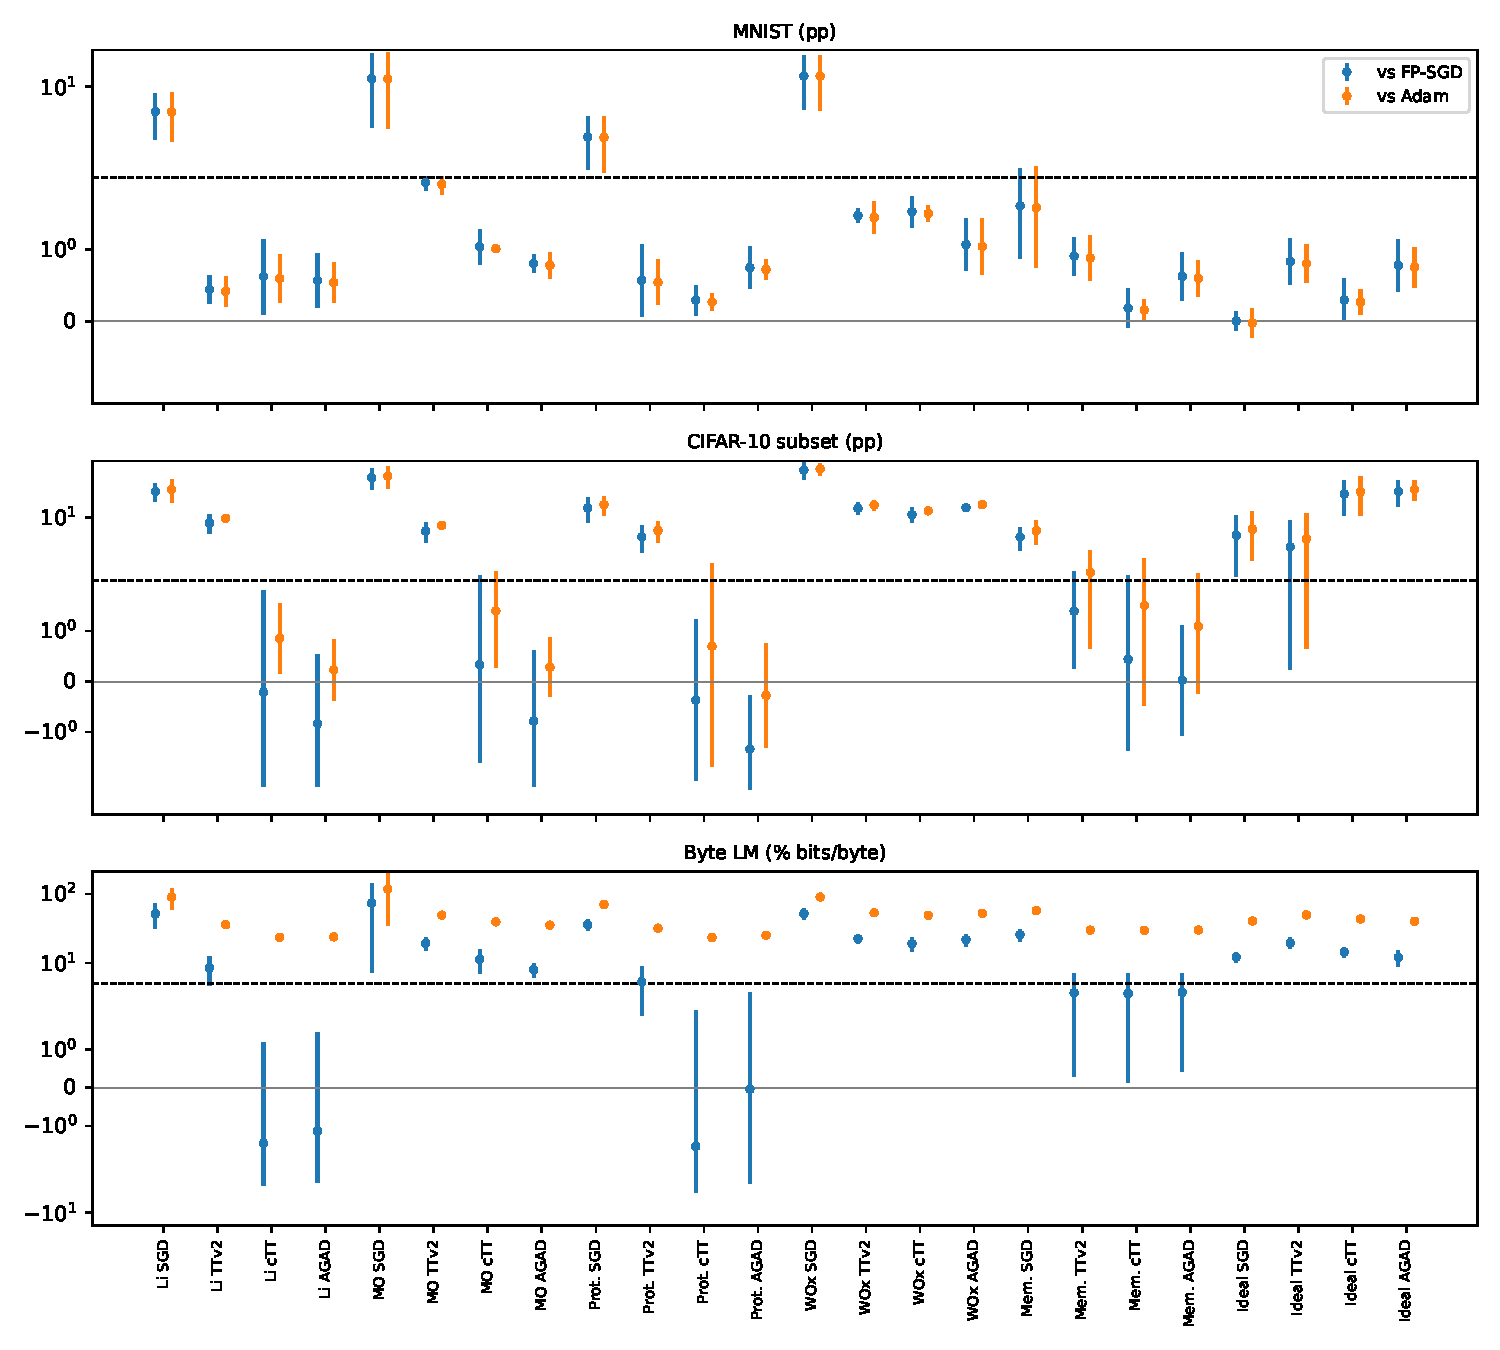
\includegraphics[width=\linewidth]{figs/fig_rev_main}
\caption{Repaired simulator: gap to FP-SGD (blue) and to digital Adam (orange) per device and algorithm, mean and 95\,\% interval
over 5 seed-matched runs (symmetric-log axis); the dashed line is the gap line.}\label{fig:rev_main}
\end{figure}
\begin{table*}[t]\centering\footnotesize\caption{Revised main table (repaired simulator): gap to FP-SGD at the same learning rate, mean [95 \% $t$-interval] over 5 seeds paired by seed (same initialisation and data order); MNIST and CIFAR in accuracy points, LM in \% of bits per byte; P/F/U = PASS/FAIL/UNRESOLVED against the absolute lines 2 pp, 2 pp, 5 \%.}\label{tab:rev_vs_fp}
\begin{tabular}{llccc}\toprule Device & Alg. & MNIST & CIFAR & LM\\\midrule
Li-ECRAM & SGD & 6.41 [3.90, 8.93] F & 19.19 [14.94, 23.44] F & 51.64 [31.63, 71.64] F\\
Li-ECRAM & TTv2 & 0.44 [0.24, 0.64] P & 8.65 [6.64, 10.66] F & 8.51 [4.72, 12.30] U\\
Li-ECRAM & c-TTv2 & 0.62 [0.10, 1.14] P & -0.21 [-2.22, 1.80] P & -1.45 [-4.07, 1.18] P\\
Li-ECRAM & AGAD & 0.57 [0.19, 0.94] P & -0.84 [-2.20, 0.53] P & -1.13 [-3.69, 1.44] P\\
MO-ECRAM & SGD & 11.51 [4.88, 18.14] F & 27.24 [20.15, 34.34] F & 73.84 [7.32, 140.36] F\\
MO-ECRAM & TTv2 & 1.93 [1.82, 2.03] U & 7.04 [5.25, 8.83] F & 19.31 [15.05, 23.57] F\\
MO-ECRAM & c-TTv2 & 1.04 [0.79, 1.28] P & 0.33 [-1.60, 2.27] U & 11.33 [7.11, 15.55] F\\
MO-ECRAM & AGAD & 0.80 [0.67, 0.93] P & -0.79 [-2.19, 0.62] P & 7.98 [6.08, 9.87] F\\
Protonic-inspired & SGD & 4.09 [2.29, 5.88] F & 12.66 [8.83, 16.49] F & 35.99 [29.87, 42.10] F\\
Protonic-inspired & TTv2 & 0.57 [0.07, 1.07] P & 6.08 [4.06, 8.10] F & 5.34 [1.89, 8.78] U\\
Protonic-inspired & c-TTv2 & 0.30 [0.09, 0.51] P & -0.37 [-1.97, 1.23] P & -1.53 [-5.07, 2.01] P\\
Protonic-inspired & AGAD & 0.75 [0.45, 1.04] P & -1.34 [-2.41, -0.27] P & -0.04 [-3.84, 3.76] P\\
W/WO$_x$ ECRAM & SGD & 12.06 [6.69, 17.42] F & 33.00 [26.34, 39.67] F & 52.03 [43.34, 60.71] F\\
W/WO$_x$ ECRAM & TTv2 & 1.47 [1.37, 1.56] P & 12.53 [10.59, 14.48] F & 22.48 [18.92, 26.04] F\\
W/WO$_x$ ECRAM & c-TTv2 & 1.52 [1.31, 1.74] P & 10.67 [8.65, 12.69] F & 19.02 [14.49, 23.55] F\\
W/WO$_x$ ECRAM & AGAD & 1.07 [0.71, 1.43] P & 12.72 [11.44, 14.01] F & 21.64 [17.52, 25.76] F\\
Memistor (optimistic) & SGD & 1.60 [0.87, 2.34] U & 6.05 [4.35, 7.75] F & 25.72 [20.59, 30.86] F\\
Memistor (optimistic) & TTv2 & 0.91 [0.64, 1.17] P & 1.39 [0.26, 2.53] U & 3.70 [0.28, 7.12] U\\
Memistor (optimistic) & c-TTv2 & 0.18 [-0.09, 0.46] P & 0.44 [-1.37, 2.25] U & 3.61 [0.14, 7.07] U\\
Memistor (optimistic) & AGAD & 0.62 [0.29, 0.96] P & 0.03 [-1.07, 1.12] P & 3.75 [0.44, 7.07] U\\
Ideal 1000-level & SGD & 0.01 [-0.12, 0.13] P & 6.32 [2.22, 10.42] F & 12.14 [10.28, 14.00] F\\
Ideal 1000-level & TTv2 & 0.83 [0.51, 1.16] P & 4.72 [0.24, 9.20] U & 19.55 [16.07, 23.03] F\\
Ideal 1000-level & c-TTv2 & 0.30 [-0.00, 0.60] P & 18.04 [10.46, 25.61] F & 14.47 [11.99, 16.96] F\\
Ideal 1000-level & AGAD & 0.78 [0.42, 1.14] P & 19.20 [13.21, 25.19] F & 12.02 [9.00, 15.03] F\\
Digital & Adam & 0.03 [-0.18, 0.23] P & -1.07 [-2.65, 0.52] P & -20.19 [-22.39, -17.99] P\\
\bottomrule\end{tabular}\end{table*}

\begin{table*}[t]\centering\footnotesize\caption{Revised main table (repaired simulator): gap to digital Adam (its own selected learning rate), mean [95 \% $t$-interval] over 5 seeds paired by seed (same initialisation and data order); MNIST and CIFAR in accuracy points, LM in \% of bits per byte; P/F/U = PASS/FAIL/UNRESOLVED against the absolute lines 2 pp, 2 pp, 5 \%.}\label{tab:rev_vs_adam}
\begin{tabular}{llccc}\toprule Device & Alg. & MNIST & CIFAR & LM\\\midrule
Li-ECRAM & SGD & 6.39 [3.79, 8.98] F & 20.25 [14.51, 26.00] F & 90.33 [60.59, 120.07] F\\
Li-ECRAM & TTv2 & 0.42 [0.21, 0.63] P & 9.72 [8.82, 10.62] F & 35.95 [34.87, 37.02] F\\
Li-ECRAM & c-TTv2 & 0.60 [0.26, 0.93] P & 0.86 [0.17, 1.55] P & 23.49 [22.61, 24.36] F\\
Li-ECRAM & AGAD & 0.54 [0.26, 0.82] P & 0.23 [-0.38, 0.84] P & 23.89 [22.95, 24.82] F\\
MO-ECRAM & SGD & 11.48 [4.73, 18.23] F & 28.31 [20.59, 36.03] F & 117.64 [35.42, 199.87] F\\
MO-ECRAM & TTv2 & 1.90 [1.77, 2.04] U & 8.11 [7.85, 8.38] F & 49.48 [47.97, 50.98] F\\
MO-ECRAM & c-TTv2 & 1.01 [0.96, 1.06] P & 1.40 [0.28, 2.53] U & 39.47 [37.39, 41.55] F\\
MO-ECRAM & AGAD & 0.78 [0.60, 0.96] P & 0.28 [-0.30, 0.86] P & 35.33 [31.48, 39.19] F\\
Protonic-inspired & SGD & 4.06 [2.18, 5.94] F & 13.73 [10.41, 17.05] F & 70.37 [65.57, 75.16] F\\
Protonic-inspired & TTv2 & 0.54 [0.23, 0.86] P & 7.15 [5.27, 9.04] F & 31.98 [30.89, 33.06] F\\
Protonic-inspired & c-TTv2 & 0.27 [0.16, 0.38] P & 0.70 [-1.68, 3.07] U & 23.36 [22.15, 24.58] F\\
Protonic-inspired & AGAD & 0.72 [0.58, 0.86] P & -0.27 [-1.30, 0.75] P & 25.23 [23.43, 27.03] F\\
W/WO$_x$ ECRAM & SGD & 12.03 [6.56, 17.50] F & 34.07 [28.80, 39.34] F & 90.44 [82.88, 97.99] F\\
W/WO$_x$ ECRAM & TTv2 & 1.44 [1.23, 1.66] P & 13.60 [11.76, 15.44] F & 53.46 [52.68, 54.24] F\\
W/WO$_x$ ECRAM & c-TTv2 & 1.50 [1.39, 1.60] P & 11.74 [10.96, 12.52] F & 49.10 [47.30, 50.90] F\\
W/WO$_x$ ECRAM & AGAD & 1.04 [0.66, 1.42] P & 13.79 [12.70, 14.88] F & 52.40 [51.04, 53.75] F\\
Memistor (optimistic) & SGD & 1.58 [0.75, 2.41] U & 7.12 [4.95, 9.30] F & 57.52 [53.05, 61.99] F\\
Memistor (optimistic) & TTv2 & 0.88 [0.57, 1.19] P & 2.46 [0.65, 4.28] U & 29.93 [28.82, 31.03] F\\
Memistor (optimistic) & c-TTv2 & 0.16 [0.01, 0.30] P & 1.51 [-0.47, 3.49] U & 29.80 [28.39, 31.22] F\\
Memistor (optimistic) & AGAD & 0.60 [0.35, 0.84] P & 1.09 [-0.24, 2.43] U & 29.99 [28.42, 31.56] F\\
Ideal 1000-level & SGD & -0.02 [-0.22, 0.18] P & 7.39 [3.31, 11.46] F & 40.53 [38.35, 42.71] F\\
Ideal 1000-level & TTv2 & 0.81 [0.54, 1.07] P & 5.79 [0.66, 10.91] U & 49.79 [48.21, 51.37] F\\
Ideal 1000-level & c-TTv2 & 0.27 [0.10, 0.44] P & 19.10 [10.33, 27.87] F & 43.45 [41.48, 45.41] F\\
Ideal 1000-level & AGAD & 0.75 [0.47, 1.03] P & 20.27 [15.32, 25.22] F & 40.36 [38.70, 42.01] F\\
\bottomrule\end{tabular}\end{table*}


\subsection{Fidelity of the aggregate update}\label{sec:fidelity}
The simulator draws each batch's pulses as independent Poisson counts per cell and applies them in one exact step of the
interleaved dynamics (Section~\ref{sec:model}). A physical stochastic-pulse array instead fires row and column lines per slot
and per sample; a cell is pulsed when both of its lines fire, and the samples follow one another. After the second review we
compared the two, pre-registered with pass lines (\texttt{PLAN-REVISION-2.md}, experiment A), on the operating regime of the
main table.

\paragraph{Update level (A1).} At two points of training, one batch's inputs, errors and array state were taken from surrogate
training runs and applied repeatedly from the same state by three methods: the surrogate; the explicit stream applied pulse by
pulse (Bernoulli line firings, the per-pulse device step, write noise and bounds after every pulse; the literal stream); and a
per-sample form of the same stream (seq), which replays the literal stream's line firings. Within one sample every pulse of a
cell has the same sign, so seq applies the sample's train in closed form. Its write noise is an approximation: it is added once
per sample at the pre-sample state (standard deviation $c_{2c}\sqrt{n}$ times the local step for $n$ pulses), and the bounds are
applied after each sample, where the literal stream applies noise and bounds after every pulse. The cases cover clipped and
unclipped layers: MNIST Li-ECRAM c-TTv2 (first and output layer), CIFAR MO-ECRAM AGAD (fully connected and output layer; the
worst-clipped layer of the main table) and the LM protonic-inspired c-TTv2 (embedding and output layer), \RYProbeN{} probes.
Version 3 compared seq with the literal stream as if their draws were independent, although they share the line firings, so
its sampling floor could hide a real difference (Table~\ref{tab:v3s_rev2_probe}, Appendix~\ref{app:revision}). The probes were
therefore run again with the draws kept, 16 per probe, and seq is now compared paired by draw, with bootstrap bounds over whole
draws (Tables~\ref{tab:rev4_probe_sur} and~\ref{tab:rev3_probe}; \texttt{PLAN-REVISION-3.md}); the draws are part of
the deposit, and Tables~\ref{tab:rev4_probe_sur}--\ref{tab:rev3_dep} can be rebuilt from them alone
(Section~\ref{sec:availability}).
\begin{itemize}
\item The surrogate, whose draws are independent of the literal stream's, meets the pre-registered lines (realised gain along
      the requested update within 10\,\%, mean difference beyond sampling noise at most 0.10, median variance ratio in
      $[0.5, 2]$) on \RYProbeSurMeetsN{} of \RYProbeN{} probes, including layers that lose up to \RYProbeOkLostMax\,\% of the
      requested pulse mass to clipping; its variance ratio lies between \RYProbeSurVarMin{} and \RYProbeSurVarMax. These are
      point estimates: with 16 draws its bootstrap bounds stay within the lines on \RYProbeSurAtNinetyFiveN{} of them.
\item It fails on the two probes of the most clipped layer: \RYProbeSurFailList. There almost nothing of the requested update
      survives the clipping, and the surrogate's Poisson counts, which can exceed the slot budget that caps the stream, no longer
      match it (review 2's limiting case: Poisson(31) exceeds 31 with probability 0.4524).
\item Paired by draw, seq meets its registered lines (gain within 5\,\%, excess at most 0.05, variance ratio in
      $[0.8, 1.25]$) on \RYProbeSeqMeetsN{} of \RYProbeN{} probes. The paired floor, \RYProbeFloorRatioMin--\RYProbeFloorRatioMax{}
      times the independent one, accounts for the raw relative difference (at most \RYProbeSeqRawMax) up to an excess of at
      most \RYProbeSeqExcessMax; gains agree within \RYProbeSeqGainDevMax\,\% and variance ratios lie in
      \RYProbeSeqVarMin--\RYProbeSeqVarMax. The bootstrap bounds stay within the lines on \RYProbeSeqAtNinetyFiveN{} probes
      (\RYProbeSeqAtNinetyFiveList). On the others (\RYProbeSeqNotNinetyFiveList) 16 draws cannot exclude a mean discrepancy of
      up to \RYProbeSeqExcessPNinetyFiveMax. Seq therefore meets our registered diagnostic thresholds; that is a diagnostic,
      not a demonstration that it is equivalent to the literal stream.
\item Shared lines make the literal stream's cells dependent; the surrogate's independent draws do not reproduce this.
      Measured by per-pair correlations, which cannot cancel (Table~\ref{tab:rev3_dep}), the root-mean-square correlation among
      cells sharing a line exceeds the surrogate's sampling null by up to \RYDepExcessMax{} (mean correlation aligned with the
      expected update's signs up to \RYDepAlignedMax), by more than 0.05 on \RYDepLargeN{} of \RYProbeN{} probes
      (\RYDepLargeList). The statistic of version 3, a pooled, signed normalised covariance, stays within \RYDepVthreePooledMax{}
      in absolute value on the same draws, because positive and negative terms cancel and unequal cell variances are pooled.
      The cross-cell dependence is therefore not small everywhere; the per-cell lines above do not test it, and whether it
      matters for training is what A2 measures.
\end{itemize}
The probes draw from a generator of their own. On the pod (version 3) the MNIST and CIFAR probe runs reproduced their main-table
records exactly; on the desk (Quadro P2200) \RYProbeRunsEqualEThree{} of \RYProbeRunsN{} do, and none shares its
initialisation with its version-3 run (the MNIST run not its example order either): the simulator's generators run on
the GPU, and the CUDA random kernels assign draws to threads by the GPU's multiprocessor count. The desk's probe runs
are therefore fresh training realisations, and the probed states are not version 3's; the comparison within each
probe is unaffected, since all three updates start from the same saved state. LM training is not bitwise reproducible even on one card
type: configurations repeated exactly in the records differ by up to \RXReproLmMaxPct\,\% in bits per byte (CIFAR
\RXReproCifarMaxPct\,\%).

\paragraph{Training level (A2).} The same selections, learning rates and seeds as the main table were trained with the
per-sample stream (MNIST: every analog layer, three devices $\times$ SGD, c-TTv2, AGAD; CIFAR: the two fully connected layers,
whose rows are one per image, for Li-ECRAM and protonic-inspired c-TTv2 and MO-ECRAM AGAD; the convolutional layers keep the
surrogate), seeds 0--2, and compared seed by seed with the main table's surrogate runs; both arms are labelled at the same three
seeds (Table~\ref{tab:rev3_fid}). The pre-registered rule calls the change material if any cell's mean gap moves by more than
half the line (1\,pp) or two cells whose gaps differ by more than 1\,pp swap order.
\begin{itemize}
\item By that rule the result is \textbf{material}, through one cell: \RXFidMaterialList, whose gap moves from
      \RXFidMnistEcramMoKimTwoZeroOneNineSgdSur{} to \RXFidMnistEcramMoKimTwoZeroOneNineSgdSeq\,pp
      (difference \RXFidMnistEcramMoKimTwoZeroOneNineSgdD\,pp, 95\,\% interval [\RXFidMnistEcramMoKimTwoZeroOneNineSgdLo,
      \RXFidMnistEcramMoKimTwoZeroOneNineSgdHi]). At three seeds both of its arms are
      \RYFidMnistEcramMoKimTwoZeroOneNineSgdSurLabel{} (surrogate [\RYFidMnistEcramMoKimTwoZeroOneNineSgdSurLo,
      \RYFidMnistEcramMoKimTwoZeroOneNineSgdSurHi], stream [\RYFidMnistEcramMoKimTwoZeroOneNineSgdSeqLo,
      \RYFidMnistEcramMoKimTwoZeroOneNineSgdSeqHi]\,pp). The rerun flagged in version 3 was done as matched triples on one GPU (experiment A2-M, Table~\ref{tab:rev4_a2m};
      \texttt{PLAN-REVISION-4.md}): on the desk's \RZAtwoMGpu, each of seeds 0--4 trained the FP-SGD control, the
      surrogate and the stream from one initialisation and one example order (equal hashes, checked; the analysis refuses
      a seed without them). At these \RZAtwoMN{} matched seeds the stream's gap is \RZAtwoMSeqGap\,pp [\RZAtwoMSeqLo,
      \RZAtwoMSeqHi], \RZAtwoMSeqLabel, against \RZAtwoMSurGap\,pp [\RZAtwoMSurLo, \RZAtwoMSurHi], \RZAtwoMSurLabel,
      with the surrogate; the paired change is \RZAtwoMD\,pp [\RZAtwoMDLo, \RZAtwoMDHi] (\RZAtwoMMaterial; its interval lies within $\pm1$\,pp). The FAIL label holds under either update.
      The pod's runs of seeds 0--2 are other random realisations of the same seeds, not a rounding variant of them: the simulator's generators run on the GPU, and the CUDA random kernels assign draws to threads by the GPU's multiprocessor count, so another GPU model draws another initialisation and example order (as predicted, the hashes differ from both the pod's and the earlier desk runs').
      Per seed the two realisations' gaps differ by up to \RZRealGapDiffMax\,pp, and at the pod's three matched seeds the
      change was \RZPodNThreeD\,pp [\RZPodNThreeDLo, \RZPodNThreeDHi]: this cell's gap depends strongly on the
      realisation, and the update's effect on it is measured only by the paired comparisons within each matched set.
      Version 4's five-seed figures for this cell mixed matched and unmatched pairs and are withdrawn (Appendix~\ref{app:revision}).
\item One label changes at the same three seeds: \RYFidTransList. Its mean gap moves by only
      \RXFidCifarEcramLiTangTwoZeroOneEightCttvTwoD\,pp, but the stream's interval
      ([\RYFidCifarEcramLiTangTwoZeroOneEightCttvTwoSeqLo, \RYFidCifarEcramLiTangTwoZeroOneEightCttvTwoSeqHi]\,pp) is wider and
      includes the line. This is not a failure, but the label is not preserved, and the difference interval
      ([\RXFidCifarEcramLiTangTwoZeroOneEightCttvTwoLo, \RXFidCifarEcramLiTangTwoZeroOneEightCttvTwoHi]\,pp) does not bound
      the change within $\pm1$\,pp.
\item \RYFidRevN{} pairs of cells reverse their mean order (\RYFidRevList); none was separated by more than 1\,pp under the
      surrogate, so there is no material rank reversal under the registered rule, but the ranking as a whole is not preserved.
      No Tiki-Taka-family cell's mean moves by more than \RXFidTtMaxAbs\,pp (MNIST at most \RXFidMnistMaxAbs\,pp including the
      SGD cell; CIFAR at most \RXFidCifarMaxAbs\,pp, with intervals of several pp at three seeds).
\end{itemize}
Within these bounds (MNIST on every layer, CIFAR on its fully connected layers, the LM at update level only, three seeds), the
registered result is one material mean change, in a failing SGD cell whose FAIL label holds at five matched seeds on one GPU under either update; no
material rank reversal; no Tiki-Taka-family mean shift above \RXFidTtMaxAbs\,pp; and one label that loses PASS. This is not a
demonstration that the surrogate and the stream train equivalently, and the per-sample stream is itself an approximation of the
literal one. The surrogate is not validated where clipping removes nearly all of the update (the CIFAR output layer above), for
the convolutional layers, or for the LM's training trajectory, and the main results remain comparisons within this
aggregate-update simulator.

% generated by revision4/analyze_rev4.py (do not edit)
\begin{table}[t]\centering\footnotesize\setlength{\tabcolsep}{3pt}\caption{Update fidelity of the aggregate surrogate against the literal pulse stream (experiment A1-P; desk rerun of A1 with the draws kept, 16 draws per probe; Li = Li-ECRAM, MO = MO-ECRAM, Prot. = protonic-inspired). Lost = requested pulse mass removed by the probability clipping (\%). The surrogate's draws are independent of the stream's, so the independent sampling floor applies: gain difference (\%, bootstrap 95 \% interval over draws), excess relative mean difference beyond the floor (bootstrap 95th percentile), median variance ratio, and whether the point estimates meet the registered lines (10 \%, 0.10, [0.5, 2]). ``(95)'': the bootstrap 95th percentile of the excess and the bootstrap 95 \% gain interval are also within their lines; it does not cover the variance ratio (a point estimate) and is not a joint 95 \% guarantee for every line.}\label{tab:rev4_probe_sur}
\fitbox{\begin{tabular}{lrrrlllc}\toprule Case & L. & Upd. & Lost & $\Delta g$ \% & excess & var. & meets\\\midrule
CIFAR MO AGAD & 3 & 600 & 36.2 & 1.4 [1.2, 1.6] & 0.06 (0.17) & 1.14 & yes\\
CIFAR MO AGAD & 4 & 600 & 95.7 & 1.5 [0.5, 2.6] & 0.15 (0.16) & 1.26 & no\\
CIFAR MO AGAD & 3 & 2000 & 26.2 & 0.5 [-0.3, 1.3] & 0.03 (0.31) & 1.07 & yes\\
CIFAR MO AGAD & 4 & 2000 & 97.3 & -4.2 [-7.8, -0.2] & 0.30 (0.32) & 1.27 & no\\
LM Prot. c-TTv2 & 0 & 750 & 6.1 & 1.3 [0.8, 1.8] & 0.03 (0.14) & 1.01 & yes\\
LM Prot. c-TTv2 & 9 & 750 & 0.0 & -0.5 [-2.4, 1.8] & 0.03 (0.32) & 0.86 & yes\\
LM Prot. c-TTv2 & 0 & 2250 & 7.0 & -0.6 [-1.0, -0.1] & 0.04 (0.13) & 1.05 & yes\\
LM Prot. c-TTv2 & 9 & 2250 & 0.0 & 0.3 [-1.8, 2.3] & 0.04 (0.32) & 0.78 & yes\\
MNIST Li c-TTv2 & 0 & 1000 & 16.0 & -0.4 [-0.8, 0.1] & 0.00 (0.14) & 1.06 & yes\\
MNIST Li c-TTv2 & 2 & 1000 & 4.6 & -1.1 [-2.6, 0.6] & 0.02 (0.10) & 1.19 & yes\\
MNIST Li c-TTv2 & 0 & 3500 & 37.5 & 0.6 [0.0, 1.1] & 0.00 (0.15) & 1.11 & yes\\
MNIST Li c-TTv2 & 2 & 3500 & 5.7 & 0.7 [-0.5, 2.1] & 0.02 (0.09) & 1.41 & yes (95)\\
\bottomrule\end{tabular}}\end{table}

% generated by revision4/analyze_rev4.py (do not edit)
\begin{table}[t]\centering\footnotesize\setlength{\tabcolsep}{3pt}\caption{Update fidelity of the per-sample stream (seq) against the literal pulse stream, paired by draw (shared line firings; experiment A1-P, the probes of Table~\ref{tab:rev4_probe_sur}): gain difference (\%, bootstrap 95 \% interval), raw relative mean difference, independent / paired sampling floor, excess beyond the PAIRED floor (bootstrap 95th percentile), median variance ratio, and whether the point estimates meet the registered lines (5 \%, 0.05, [0.8, 1.25]). ``(95)'': the bootstrap 95th percentile of the excess and the bootstrap 95 \% gain interval are also within their lines; it does not cover the variance ratio (a point estimate) and is not a joint 95 \% guarantee for every line.}\label{tab:rev3_probe}
\fitbox{\begin{tabular}{lrrlllllc}\toprule Case & L. & Upd. & $\Delta g$ \% & raw & floor ind./pair. & excess & var. & meets\\\midrule
CIFAR MO AGAD & 3 & 600 & 0.1 [-0.1, 0.2] & 0.114 & 0.121 / 0.114 & 0.011 (0.144) & 1.00 & yes\\
CIFAR MO AGAD & 4 & 600 & -0.9 [-1.5, -0.3] & 0.050 & 0.050 / 0.050 & 0.005 (0.064) & 1.03 & yes\\
CIFAR MO AGAD & 3 & 2000 & -0.2 [-0.6, 0.1] & 0.224 & 0.241 / 0.224 & 0.015 (0.286) & 1.00 & yes\\
CIFAR MO AGAD & 4 & 2000 & -1.4 [-5.5, 3.5] & 0.072 & 0.074 / 0.073 & 0.000 (0.094) & 1.00 & yes\\
LM Prot. c-TTv2 & 0 & 750 & -0.0 [-0.2, 0.2] & 0.032 & 0.106 / 0.032 & 0.000 (0.041) & 1.00 & yes (95)\\
LM Prot. c-TTv2 & 9 & 750 & 0.0 [-0.3, 0.3] & 0.075 & 0.258 / 0.075 & 0.000 (0.095) & 1.00 & yes\\
LM Prot. c-TTv2 & 0 & 2250 & 0.1 [-0.0, 0.3] & 0.029 & 0.093 / 0.028 & 0.004 (0.037) & 1.00 & yes (95)\\
LM Prot. c-TTv2 & 9 & 2250 & 0.2 [-0.2, 0.5] & 0.073 & 0.249 / 0.073 & 0.007 (0.093) & 1.00 & yes\\
MNIST Li c-TTv2 & 0 & 1000 & -0.0 [-0.0, 0.0] & 0.036 & 0.109 / 0.036 & 0.001 (0.045) & 1.00 & yes (95)\\
MNIST Li c-TTv2 & 2 & 1000 & 0.1 [-0.1, 0.2] & 0.027 & 0.074 / 0.027 & 0.000 (0.035) & 1.02 & yes (95)\\
MNIST Li c-TTv2 & 0 & 3500 & -0.0 [-0.1, 0.0] & 0.036 & 0.113 / 0.036 & 0.003 (0.046) & 1.00 & yes (95)\\
MNIST Li c-TTv2 & 2 & 3500 & 0.1 [-0.2, 0.3] & 0.024 & 0.063 / 0.025 & 0.000 (0.031) & 0.99 & yes (95)\\
\bottomrule\end{tabular}}\end{table}

% generated by revision4/analyze_rev4.py (do not edit)
\begin{table*}[t]\centering\footnotesize\setlength{\tabcolsep}{3pt}\caption{Cross-cell dependence of the literal stream's draws (experiment A1-P), among cells sharing a row / a column, from per-pair Pearson correlations over all pairs (they cannot cancel): root-mean-square correlation of the literal stream and of the surrogate (whose cells are independent, so its value is the sampling null at the same number of draws), the excess RMS beyond that null, taken in quadrature ($\sqrt{\max(0,\,\mathrm{RMS}_{\mathrm{slot}}^2-\mathrm{RMS}_{\mathrm{null}}^2)}$), the mean correlation aligned with the signs of the expected update, the largest per-line RMS, and the version-3 statistic (a pooled, signed normalised covariance, which can cancel).}\label{tab:rev3_dep}
\fitbox{\begin{tabular}{lrrcccccc}\toprule Case & L. & Upd. & RMS slot & RMS sur.\ (null) & excess RMS & aligned mean & max line RMS & v3 pooled\\\midrule
CIFAR MO AGAD & 3 & 600 & 0.258 / 0.261 & 0.258 / 0.258 & 0.009 / 0.041 & 0.005 / 0.010 & 0.262 / 1.000 & 0.000 / -0.000\\
CIFAR MO AGAD & 4 & 600 & 0.256 / 0.261 & 0.259 / 0.260 & 0.000 / 0.026 & 0.007 / -0.004 & 0.259 / 0.645 & 0.000 / -0.008\\
CIFAR MO AGAD & 3 & 2000 & 0.260 / 0.260 & 0.258 / 0.258 & 0.032 / 0.026 & 0.007 / 0.004 & 0.283 / 0.399 & -0.000 / -0.000\\
CIFAR MO AGAD & 4 & 2000 & 0.259 / 0.260 & 0.259 / 0.255 & 0.015 / 0.048 & 0.006 / -0.003 & 0.265 / 0.315 & 0.000 / 0.001\\
LM Prot. c-TTv2 & 0 & 750 & 0.259 / 0.258 & 0.258 / 0.258 & 0.015 / 0.008 & -0.000 / 0.000 & 0.266 / 0.264 & 0.000 / 0.000\\
LM Prot. c-TTv2 & 9 & 750 & 0.299 / 0.258 & 0.258 / 0.258 & 0.152 / 0.007 & 0.026 / -0.000 & 1.000 / 0.264 & -0.000 / -0.001\\
LM Prot. c-TTv2 & 0 & 2250 & 0.258 / 0.258 & 0.258 / 0.258 & 0.000 / 0.000 & -0.000 / 0.000 & 0.265 / 0.262 & 0.000 / -0.000\\
LM Prot. c-TTv2 & 9 & 2250 & 0.315 / 0.258 & 0.258 / 0.258 & 0.180 / 0.003 & 0.025 / -0.000 & 1.000 / 0.266 & 0.001 / -0.001\\
MNIST Li c-TTv2 & 0 & 1000 & 0.335 / 0.262 & 0.258 / 0.258 & 0.213 / 0.044 & 0.054 / 0.010 & 0.454 / 0.589 & -0.000 / -0.000\\
MNIST Li c-TTv2 & 2 & 1000 & 0.399 / 0.262 & 0.258 / 0.260 & 0.305 / 0.031 & 0.103 / 0.014 & 0.494 / 0.348 & -0.000 / -0.020\\
MNIST Li c-TTv2 & 0 & 3500 & 0.385 / 0.259 & 0.258 / 0.258 & 0.286 / 0.025 & 0.100 / 0.004 & 0.478 / 0.322 & -0.001 / -0.000\\
MNIST Li c-TTv2 & 2 & 3500 & 0.431 / 0.264 & 0.258 / 0.258 & 0.345 / 0.057 & 0.208 / 0.003 & 0.522 / 0.321 & 0.006 / -0.003\\
\bottomrule\end{tabular}}\end{table*}

% generated by revision4/analyze_rev4.py (do not edit)
\begin{table}[t]\centering\footnotesize\setlength{\tabcolsep}{3pt}\caption{Experiment A2-M: MNIST MO-ECRAM SGD as matched triples on one GPU (Quadro P2200): per seed, the FP-SGD control's, the surrogate's and the per-sample stream's test accuracy (\%) and the two gaps to the control (pp); every seed's three runs share their initialisation and example order (equal hashes, checked). Right: the same seeds' gaps from the pod's matched triples (RTX A4000), a different random realisation of each seed.}\label{tab:rev4_a2m}
\fitbox{\begin{tabular}{rrrrllll}\toprule & \multicolumn{5}{c}{P2200} & \multicolumn{2}{c}{pod (A4000)}\\\cmidrule(lr){2-6}\cmidrule(lr){7-8} Seed & FP-SGD & sur. & seq & gap sur. & gap seq & gap sur. & gap seq\\\midrule
0 & 97.90 & 89.83 & 90.02 & 8.07 & 7.88 & 16.84 & 15.69\\
1 & 97.60 & 87.86 & 87.30 & 9.74 & 10.30 & 7.59 & 7.39\\
2 & 97.68 & 89.79 & 90.26 & 7.89 & 7.42 & 17.86 & 14.95\\
3 & 97.74 & 87.20 & 87.22 & 10.54 & 10.52 & -- & --\\
4 & 97.75 & 90.44 & 90.20 & 7.31 & 7.55 & -- & --\\
\midrule mean [95\,\%] & & & & 8.71 [7.02, 10.40] & 8.73 [6.82, 10.65] & & \\
\bottomrule\end{tabular}}\end{table}

% generated by revision3/analyze_rev3.py (do not edit)
\begin{table*}[t]\centering\footnotesize\caption{Training fidelity (experiment A2), seeds 0--2 on both arms: mean gap to FP-SGD (pp) with its 95 \% interval and label against the 2\,pp line (P pass, U unresolved, F fail), with the aggregate surrogate (E3's records) and with the per-sample pulse stream (MNIST: every analog layer; CIFAR: the two fully connected layers); the paired difference with its 95 \% interval; material by the registered rule (|mean| $>$ 1\,pp). The labels are at $n=3$; the main table's labels are at $n=5$.}\label{tab:rev3_fid}
\fitbox{\begin{tabular}{lllll c}\toprule Task & Cell & surrogate & stream & difference & material\\\midrule
CIFAR & Li-ECRAM c-TTv2 & -1.14 [-3.89, 1.62] P & -0.62 [-6.44, 5.20] U & 0.52 [-3.26, 4.29] & no\\
CIFAR & MO-ECRAM AGAD & -1.40 [-3.22, 0.41] P & -1.82 [-3.76, 0.13] P & -0.41 [-1.99, 1.16] & no\\
CIFAR & Protonic-inspired c-TTv2 & -0.85 [-3.33, 1.64] P & -1.46 [-3.94, 1.02] P & -0.61 [-2.86, 1.64] & no\\
MNIST & Li-ECRAM AGAD & 0.65 [-0.26, 1.56] P & 0.49 [0.08, 0.90] P & -0.16 [-0.69, 0.36] & no\\
MNIST & Li-ECRAM c-TTv2 & 0.68 [-0.77, 2.12] U & 0.74 [-1.70, 3.18] U & 0.07 [-0.95, 1.09] & no\\
MNIST & Li-ECRAM SGD & 6.99 [0.52, 13.46] U & 6.90 [1.03, 12.76] U & -0.09 [-0.73, 0.54] & no\\
MNIST & MO-ECRAM AGAD & 0.77 [0.48, 1.06] P & 0.89 [0.70, 1.07] P & 0.11 [-0.07, 0.30] & no\\
MNIST & MO-ECRAM c-TTv2 & 1.08 [0.44, 1.72] P & 1.05 [0.43, 1.66] P & -0.04 [-0.23, 0.16] & no\\
MNIST & MO-ECRAM SGD & 14.10 [0.04, 28.15] U & 12.68 [1.27, 24.09] U & -1.42 [-4.84, 2.00] & yes\\
MNIST & Protonic-inspired AGAD & 0.79 [0.15, 1.43] P & 0.77 [0.17, 1.37] P & -0.02 [-0.39, 0.35] & no\\
MNIST & Protonic-inspired c-TTv2 & 0.29 [-0.30, 0.88] P & 0.21 [-0.71, 1.13] P & -0.08 [-0.44, 0.27] & no\\
MNIST & Protonic-inspired SGD & 4.58 [0.15, 9.00] U & 4.69 [0.01, 9.38] U & 0.12 [-0.33, 0.56] & no\\
\bottomrule\end{tabular}}\end{table*}


\subsection{Width}\label{sec:scale}
An earlier lane of this project saw the device gap grow with model width. Here every arm (protonic-inspired and Li-ECRAM, each
with TTv2 and c-TTv2) gets its own learning rate at every width by the edge rule on validation, and then five test seeds per
width; FP-SGD uses its own selected rate (Table~\ref{tab:rev_width}; the rates are in Table~\ref{tab:rev_selection}). As in the
rest of the paper, each layer's weight scale $\alpha$ is set from its initialisation bound, so it falls as $1/\sqrt{\text{fan-in}}$
when the width raises a layer's fan-in (layers with a fixed fan-in keep theirs); this is one mapping policy, not every fixed
physical mapping.

\paragraph{The test.} The endpoint contrast $D$ (the mean gap at the widest minus the narrowest width) is tested for
equivalence within the gap lines (TOST at 5\,\%). The original paper's ``FLAT'' label is withdrawn: it did not test equivalence
and covered large non-monotonic changes. The pre-registered contrast is Welch's, which treats the two widths' seed samples as
independent. They are not: every arm of a seed shares the logical initialisation and the data order across widths. Beside the
registered result we therefore report the contrast paired by seed, with the same decision order, as a sensitivity analysis
added after the second review (deviation R4). Both test the endpoints only; neither covers the middle width.

\paragraph{CIFAR ($c=16$, 32, 64).} \RVEFourCifarNEquivalent{} arm is equivalent within $\pm2$\,pp (Li-ECRAM c-TTv2,
$D=\RVEFourCifarEcramLiTangTwoZeroOneEightCttvTwoD$\,pp, 90\,\% interval [\RVEFourCifarEcramLiTangTwoZeroOneEightCttvTwoLo,
\RVEFourCifarEcramLiTangTwoZeroOneEightCttvTwoHi]); for \RVEFourCifarNNoEvidenceOfGrowthBeyondTheMargin{} arm there is no evidence
of growth beyond the margin (protonic-inspired TTv2); \RVEFourCifarNInconclusive{} arms are inconclusive (Li-ECRAM TTv2,
$D=\RVEFourCifarEcramLiTangTwoZeroOneEightTtvTwoD$\,pp; protonic-inspired c-TTv2, $D=\RVEFourCifarProtonicOnenTwoZeroTwoTwoCttvTwoD$\,pp).
Five seeds are not enough to settle a 2\,pp margin on this subset. Paired by seed, the Li-ECRAM c-TTv2 equivalence survives
(90\,\% interval [\RVEFourCifarEcramLiTangTwoZeroOneEightCttvTwoPairedLo, \RVEFourCifarEcramLiTangTwoZeroOneEightCttvTwoPairedHi]),
and protonic-inspired c-TTv2 \emph{grows} ([\RVEFourCifarProtonicOnenTwoZeroTwoTwoCttvTwoPairedLo,
\RVEFourCifarProtonicOnenTwoZeroTwoTwoCttvTwoPairedHi]): the growth is detected, but its size against the margin is
unresolved: the interval includes 2\,pp, so growth beyond the margin is not excluded. Both of its
endpoint cells still pass against their own FP-SGD controls; a gap that moves from more negative to less negative can grow while
both cells stay acceptable. Li-ECRAM TTv2 stays inconclusive, so growth beyond the margin is not excluded for it either.

\paragraph{The LM ($d=64$, 128, 256).} All \RVEFourLmNShrinks{} arms have a gap that shrinks with width (for example Li-ECRAM
c-TTv2 from \RVEFourLmEcramLiTangTwoZeroOneEightCttvTwoWSixFourGap\,\% to \RVEFourLmEcramLiTangTwoZeroOneEightCttvTwoWTwoFiveSixGap\,\%).
This is not a favourable scaling law: FP-SGD itself gets worse at the largest width under the fixed budget
(\RVEFourLmFpWOneTwoEight{} bits per byte at $d=128$, \RVEFourLmFpWTwoFiveSix{} at $d=256$), so a gap that turns negative partly
measures a weaker baseline. Converged or quality-matched baselines would be needed to speak of scaling.

\paragraph{What can be said.} Across a factor of four in width, after per-arm learning-rate selection, no arm's gap grows
detectably beyond the margin. Endpoint equivalence is established for one CIFAR arm only (Li-ECRAM c-TTv2, by both contrasts);
the paired analysis detects growth for one other CIFAR arm (protonic-inspired c-TTv2), which the registered Welch test
does not, without resolving its size against the margin; for \RYWidthNotExcludedN{} arms (protonic-inspired c-TTv2 and
Li-ECRAM TTv2) growth beyond the margin is not excluded. On the LM the apparent shrinkage reflects the FP-SGD
baseline at a fixed budget. Width dependence is unresolved by this study.

\begin{table*}[t]\centering\scriptsize\caption{Revised width study (Li = Li-ECRAM, Prot. = protonic-inspired): mean gap at the narrow / mid / wide width (5 seeds, each arm at its own selected learning rate; CIFAR $c=16/32/64$ in pp, LM $d=64/128/256$ in \%), and the endpoint contrast $D$ (widest minus narrowest) with its 90 \% interval and verdict, by the pre-registered Welch test (the $t$ quantile at the Welch--Satterthwaite degrees of freedom; versions 2--11 rounded them down: deviation R9) and, added after review 2 (deviation R4), paired by seed. Verdicts (margins 2 pp, 5 \%): EQ = equivalent at the endpoints, GR = grows, SH = shrinks, NG = no evidence of growth beyond the margin, INC = inconclusive. An endpoint test says nothing about the middle width.}\label{tab:rev_width}
\begin{tabular}{llccc}\toprule Task & Arm & gap narrow / mid / wide & Welch $D$ [90 \%] & paired $D$ [90 \%]\\\midrule
CIFAR & Li c-TTv2 & -0.36 / 0.66 / -0.71 & -0.34 [-1.34, 0.65] EQ & -0.34 [-1.79, 1.11] EQ\\
CIFAR & Li TTv2 & 3.29 / 4.12 / 5.20 & 1.91 [-0.34, 4.16] INC & 1.91 [-1.53, 5.35] INC\\
CIFAR & Prot. c-TTv2 & -2.57 / -1.55 / -0.81 & 1.76 [0.05, 3.47] GR & 1.76 [0.15, 3.38] GR\\
CIFAR & Prot. TTv2 & 1.38 / 2.71 / 0.43 & -0.95 [-2.51, 0.60] NG & -0.95 [-3.36, 1.46] NG\\
LM & Li c-TTv2 & 1.21 / -4.69 / -12.90 & -14.12 [-15.37, -12.87] SH & -14.12 [-15.30, -12.94] SH\\
LM & Li TTv2 & 9.85 / 13.29 / -3.07 & -12.92 [-14.55, -11.29] SH & -12.92 [-14.99, -10.85] SH\\
LM & Prot. c-TTv2 & -5.79 / -6.36 / -12.69 & -6.90 [-8.08, -5.72] SH & -6.90 [-7.76, -6.04] SH\\
LM & Prot. TTv2 & 7.95 / 0.39 / -6.49 & -14.44 [-19.12, -9.75] SH & -14.44 [-19.31, -9.57] SH\\
\bottomrule\end{tabular}\end{table*}


\subsection{Sensitivity against absolute lines}\label{sec:spec}
% derived by revision4/edit_tex_4b.py from tables/rev_spec.tex: placement [p] instead of [t]
\begin{table*}[p]\centering\scriptsize\caption{Revised sensitivity sheet (protonic-inspired base; TTv2 = the pre-registered S-ALGO, c-TTv2 added after the main table was seen, deviation R3; 3 seeds paired with FP-SGD): mean gap per grid value with its label against the ABSOLUTE line (P/F/U), and the weakest value that passes with every value toward the best end also passing (-- = not established).}\label{tab:rev_spec}
\begin{tabular}{llp{8.8cm}l}\toprule Alg., task & Axis & mean gap per value & threshold\\\midrule
c-TTv2, CIFAR & levels & 5000.0: 2.49U; 2000.0: -2.43P; 1000: -0.85P; 500.0: -1.57P; 200.0: 1.38U; 100.0: 1.68U & --\\
c-TTv2, CIFAR & asym.\ $a$ (SP moves) & 0.0: -1.43P; 0.05: -0.85P; 0.1: -1.64P; 0.2: -1.16P; 0.4: 42.39F & 0.2\\
c-TTv2, CIFAR & asym.\ $a$ (SP fixed) & 0.0: -1.43P; 0.05: -0.41P; 0.1: -0.82U; 0.2: -1.38U; 0.4: -0.53U & 0.05\\
c-TTv2, CIFAR & nonlin.\ $\gamma$ & 0.0: 21.14F; 0.2: -0.85P; 0.5: 1.88U; 1.0: 8.01F; 2.0: 14.77F & --\\
c-TTv2, CIFAR & noise $c_{2c}$ & 0.0: -0.64U; 0.3: -0.85P; 1.0: -1.34U; 2.0: 0.61U; 4.0: 5.37U & --\\
c-TTv2, CIFAR & ref.\ err.\ $\sigma_r$ & 0.0: -1.20P; 0.02: -0.85P; 0.05: -1.29P; 0.1: 2.89U; 0.2: 9.31F; 0.5: 34.63F & 0.05\\
c-TTv2, CIFAR & retention $\tau$ & inf: -0.85P; 100000.0: -1.17U; 10000.0: 3.08U; 1000.0: 33.02F; 100.0: 44.03F & inf\\
c-TTv2, LM & levels & 5000.0: 2.01U; 2000.0: -2.63U; 1000: -1.84U; 500.0: -0.45U; 200.0: 1.58U; 100.0: 6.54U & --\\
c-TTv2, LM & asym.\ $a$ (SP moves) & 0.0: -1.68U; 0.05: -1.84U; 0.1: -1.54U; 0.2: -1.85U; 0.4: 37.71U & --\\
c-TTv2, LM & asym.\ $a$ (SP fixed) & 0.0: -1.62U; 0.05: -2.16U; 0.1: -1.69U; 0.2: -1.70U; 0.4: -1.68U & --\\
c-TTv2, LM & nonlin.\ $\gamma$ & 0.0: 22.71F; 0.2: -1.84U; 0.5: -0.39U; 1.0: 4.46U; 2.0: 27.27U & --\\
c-TTv2, LM & noise $c_{2c}$ & 0.0: -1.51U; 0.3: -1.84U; 1.0: -0.21U; 2.0: 4.91U; 4.0: 19.04F & --\\
c-TTv2, LM & ref.\ err.\ $\sigma_r$ & 0.0: -2.42U; 0.02: -1.84U; 0.05: 1.45U; 0.1: 8.23U; 0.2: 17.53F; 0.5: 30.83F & --\\
c-TTv2, LM & retention $\tau$ & inf: -1.84U; 100000.0: -1.75U; 10000.0: -3.47U; 1000.0: 28.50F; 100.0: 64.34F & --\\
TTv2, CIFAR & levels & 5000.0: 0.78U; 2000.0: 1.67U; 1000: 6.35U; 500.0: 4.43U; 200.0: 3.13U; 100.0: 3.12U & --\\
TTv2, CIFAR & asym.\ $a$ (SP moves) & 0.0: 5.92U; 0.05: 6.35U; 0.1: 5.95F; 0.2: 6.39F; 0.4: 42.92F & --\\
TTv2, CIFAR & asym.\ $a$ (SP fixed) & 0.0: 5.92U; 0.05: 6.02U; 0.1: 6.12U; 0.2: 4.60U; 0.4: 6.20U & --\\
TTv2, CIFAR & nonlin.\ $\gamma$ & 0.0: 27.43F; 0.2: 6.35U; 0.5: 9.00F; 1.0: 8.22F; 2.0: 12.20F & --\\
TTv2, CIFAR & noise $c_{2c}$ & 0.0: 5.79U; 0.3: 6.35U; 1.0: 6.19U; 2.0: 7.18U; 4.0: 9.40F & --\\
TTv2, CIFAR & ref.\ err.\ $\sigma_r$ & 0.0: 5.08U; 0.02: 6.35U; 0.05: 5.35U; 0.1: 9.94F; 0.2: 18.74F; 0.5: 30.32F & --\\
TTv2, CIFAR & retention $\tau$ & inf: 6.35U; 100000.0: 4.49U; 10000.0: 5.18U; 1000.0: 40.83F; 100.0: 47.25F & --\\
TTv2, LM & levels & 5000.0: 7.33U; 2000.0: 4.67U; 1000: 5.15U; 500.0: 5.87U; 200.0: 7.38U; 100.0: 9.64U & --\\
TTv2, LM & asym.\ $a$ (SP moves) & 0.0: 5.26U; 0.05: 5.15U; 0.1: 5.21U; 0.2: 5.00U; 0.4: 10.38U & --\\
TTv2, LM & asym.\ $a$ (SP fixed) & 0.0: 5.25U; 0.05: 5.15U; 0.1: 5.28U; 0.2: 5.29U; 0.4: 5.75U & --\\
TTv2, LM & nonlin.\ $\gamma$ & 0.0: 32.24F; 0.2: 5.15U; 0.5: 11.13U; 1.0: 18.03F; 2.0: 25.84F & --\\
TTv2, LM & noise $c_{2c}$ & 0.0: 5.14U; 0.3: 5.15U; 1.0: 5.56U; 2.0: 7.85U; 4.0: 15.03U & --\\
TTv2, LM & ref.\ err.\ $\sigma_r$ & 0.0: 4.59U; 0.02: 5.15U; 0.05: 7.27U; 0.1: 11.43U; 0.2: 19.66F; 0.5: 31.81F & --\\
TTv2, LM & retention $\tau$ & inf: 5.15U; 100000.0: 5.09U; 10000.0: 3.74U; 1000.0: 30.34F; 100.0: 71.47F & --\\
\bottomrule\end{tabular}\end{table*}

Around the protonic-inspired base we move one device property at a time (levels, step asymmetry, saturation $\gamma$, write
noise, reference error, retention) at the base sizes (CIFAR $c=32$, LM $d=128$), three seeds paired with FP-SGD of the same seed,
at FP-SGD's learning rate. Every grid point is labelled against the \emph{absolute} line (2\,pp, 5\,\%), never against the base
device's own gap (Table~\ref{tab:rev_spec}). The asymmetry sweep is run twice: as before, where the symmetry point
$u^*=a/(2\gamma)$ moves toward the upper bound and the positive weight range shrinks ($a=0.4$ at $\gamma=0.2$ puts $u^*$ on the
bound); and with each device's range re-centred on its symmetry point, so that only the up/down dynamics change.

\paragraph{The pre-registered sheet (TTv2) establishes no threshold.} Its base point is itself UNRESOLVED on both tasks
(\RVSpecTtvTwoCifarBaseGap\,pp on CIFAR, \RVSpecTtvTwoLmBaseGap\,\% on the LM), so by the pre-registered rule every axis is ``not
established''. It still shows the confound the review pointed out: at $a=0.4$ the gap is \RVSpecTtvTwoCifarAsymAtZeroPFourGap\,pp
on CIFAR when the symmetry point moves onto the bound, but \RVSpecTtvTwoCifarAsymFixedspAtZeroPFourGap\,pp when it is held at
mid-range. The earlier ``asymmetry limit'' was mostly lost weight range.

\paragraph{The chopped-TTv2 sheet (added after the main table, deviation R3).} On CIFAR the base passes
(\RVSpecCttvTwoCifarBaseGap\,pp, \RVSpecCttvTwoCifarBaseLabel), and the sheet establishes: step asymmetry up to
\RVSpecCttvTwoCifarAsymThr{} with the symmetry point moving (at 0.4 the gap jumps to \RVSpecCttvTwoCifarAsymAtZeroPFourGap\,pp,
when $u^*$ reaches the bound), and reference error up to \RVSpecCttvTwoCifarRefErrThr{} of the half range. With the symmetry point
held at mid-range, version 2 borrowed the ordinary base (whose range is $[-1.125, +0.875]$) as this sweep's anchor and omitted
its zero point (deviation R5); both are now run with each device's range re-centred (range $[-1, 1]$, pre-registered after the
second review). The recentred base passes (\RVSpecCttvTwoCifarAsymFixedspAtZeroPZeroFiveGap\,pp) and so does $a=0$
(\RVSpecCttvTwoCifarAsymFixedspAtZeroPZeroGap\,pp), so the held-symmetry threshold \RVSpecCttvTwoCifarAsymFixedspThr{} is now
established by its own runs; it differs from the unrecentred base by \RXFixCttvTwoCifarRmu\,pp (95\,\% interval
[\RXFixCttvTwoCifarRmuLo, \RXFixCttvTwoCifarRmuHi]). No point fails: up to $a=0.4$ the mean gap stays at
\RVSpecCttvTwoCifarAsymFixedspAtZeroPFourGap\,pp and the intervals merely include the line. Levels,
saturation, write noise and finite retention are not established: neighbouring grid values are UNRESOLVED with three seeds,
while the clear failures are no saturation ($\gamma=0$: \RVSpecCttvTwoCifarGammaAtZeroPZeroGap\,pp), strong saturation
($\gamma=1$: \RVSpecCttvTwoCifarGammaAtOnePZeroGap\,pp), reference error 0.2 (\RVSpecCttvTwoCifarRefErrAtZeroPTwoGap\,pp) and
retention of $10^3$ updates or less. On the LM the base is \RVSpecCttvTwoLmBaseLabel{} with three seeds
(\RVSpecCttvTwoLmBaseGap\,\%; it passed with five seeds in the main table), so no LM threshold is established.

\paragraph{How to read the sheet.} These are one-at-a-time ranges around one base device, for one algorithm setting, at FP-SGD's
learning rate, with three seeds; they are exploratory, not fabrication tolerances. Combined deviations, other algorithm
settings and independent device populations are not covered. A near-zero saturation fails here because, with these settings,
the accumulator's decay comes from the device (Section~\ref{sec:main}); it is not a general requirement for training. The rule
is deliberately stringent: an UNRESOLVED point at the best end of an axis blocks a threshold even where intermediate points pass.
``Not established'' therefore does not mean that no grid value passed (on CIFAR with c-TTv2 the 500, 1000 and 2000 level points
pass, \RVSpecCttvTwoCifarNStatesAtFiveZeroZeroPZeroGap, \RVSpecCttvTwoCifarNStatesAtOneZeroZeroZeroGap{} and
\RVSpecCttvTwoCifarNStatesAtTwoZeroZeroZeroPZeroGap\,pp, while 5000 levels give \RVSpecCttvTwoCifarNStatesAtFiveZeroZeroZeroPZeroGap\,pp,
UNRESOLVED), and it does not show that more levels harm hardware training in general.



\section{A conditional energy projection for the weight-matrix operations}\label{sec:energy}
This section is an accounting scenario, not an energy measurement of a training system. It asks how much energy the
weight-matrix operations of a training step would take if the analog reads ran at the efficiency of a published analog-AI
\emph{inference} chip and the updates cost the published or projected pulse energies, and it compares that with an H100.

\paragraph{Assumptions, stated first.}
\begin{enumerate}
\item \textbf{Different read assumptions for accuracy and energy.} The accuracies of Section~\ref{sec:main} are simulated with
      ideal fp32 reads; the energy prices finite-precision analog reads. We have not shown that one operating point gives both
      the reported accuracy and the assumed read efficiency.
\item \textbf{The read efficiency is borrowed from a phase-change inference chip}~\cite{ambrogio2023}: up to 12.4\,TOPS/W
      sustained, measured on one chip, and 6.94\,TOPS/W, the authors' \emph{projected} full-system figure for their five-chip
      system: the chips were not integrated with digital processing, whose time and energy the authors estimate from their
      architecture model, and external components such as system buses and voltage regulators are excluded. We report both. Neither is an ECRAM training array, which also needs
      backward reads, repeated writes, references and Tiki-Taka state.
\item \textbf{The boundary is the weight matrices.} Per weight and per training row: the forward and backward reads (two MACs)
      and the update (device pulses, pulse lines and pulse generation, and the TT family's column reads and digital buffer).
      Attention products, nonlinearities, normalisation, activation storage, data movement, control, reference maintenance and
      static power are not modelled on either side, and the digital exclusions do not cancel the analog ones.
\item \textbf{The GPU side} is H100 board power over its dense BF16 peak~\cite{nvidiah100} at the utilisation of a very large
      training run, 38--43\,\%~\cite{dubey2024}: \RVenGpuPj\,pJ per weight per row (\RVenGpuMeasLo--\RVenGpuMeasHi\,pJ over that
      range; \RVenGpuPlannedLo--\RVenGpuPlannedHi\,pJ over the 30--55\,\% range of our original plan).
\end{enumerate}

\paragraph{Projection.} With the repaired pulse counts (resets counted as applied, the pulse reset's extra reads included), the
GPU-to-analog ratio per weight per row is \RVenChipMin--\RVenChipMax$\times$ at the 12.4\,TOPS/W chip figure and
\RVenSysMin--\RVenSysMax$\times$ at the 6.94\,TOPS/W system figure, for every published device and algorithm. The reads are at
least \RVenChipMvmShareMin\,\% of the analog total: the ratio is set almost entirely by the two borrowed efficiencies, and
changes in the simulated pulse counts barely move it.

\paragraph{Conditional ratios for cells that pass the margin.} A low energy per operation is worth nothing without the
accuracy. PASS means that the whole confidence interval of the gap lies within the stated non-inferiority margin under ideal reads,
not that the losses are equal; we therefore print the ratio only for cells that PASS against the stated baseline
(Table~\ref{tab:rev_energy}), mark FAIL cells as missing the margin and UNRESOLVED cells as ``criterion not established'':
\begin{itemize}
\item against FP-SGD: \RVenEqFpMnistN, \RVenEqFpCifarN{} and \RVenEqFpLmN{} of the \RVenCellsMnistN{} published-device cells per
      task (MNIST, CIFAR, LM);
\item against Adam: \RVenEqAdamMnistN, \RVenEqAdamCifarN{} and \RVenEqAdamLmN{} cells. \textbf{On the LM no analog cell passes
      the margin against Adam, so no conditional ratio exists against the stronger digital baseline.}
\end{itemize}
The comparison is at a fixed training budget; reaching a quality at a different number of steps is not modelled. No joint
finite-read operating point of accuracy and energy, and no energy-to-target training trajectory, is demonstrated; finite
precision, tiling and utilisation, reference maintenance, the digital TT state, update scheduling and full-system costs stay
outside the ratio.

\paragraph{What 100$\times$ would need.} At the central GPU figure, a 100$\times$ ratio needs reads at about
\RVenNeedTopsMin--\RVenNeedTopsMax\,TOPS/W including their periphery, several times the chip figure above.

\paragraph{The memistor.} Widrow's macroscopic memistor moves tens of microjoules of plating charge per level; its ratio is at
most \RVenWidrowRatioMax{} (far worse than the GPU), as expected for wet, centimetre-scale cells.

\begin{table*}[t]\centering\scriptsize\caption{Conditional energy ratios for cells that pass the stated non-inferiority margin under ideal reads: the GPU-to-analog energy ratio per weight per row (12.4 TOPS/W measured chip figure / 6.94 TOPS/W projected system figure of the same inference chip, which includes estimated digital processing), printed only where the cell PASSES against the baseline; fail = the cell FAILS the margin; n.e. = the criterion is not established (UNRESOLVED). No finite-read operating point is demonstrated.}\label{tab:rev_energy}
\begin{tabular}{llcccccc}\toprule & & \multicolumn{2}{c}{MNIST} & \multicolumn{2}{c}{CIFAR} & \multicolumn{2}{c}{LM}\\ Device & Alg. & FP-SGD & Adam & FP-SGD & Adam & FP-SGD & Adam\\\midrule
Li-ECRAM & SGD & fail & fail & fail & fail & fail & fail\\
Li-ECRAM & TTv2 & 32 / 18 & 32 / 18 & fail & fail & n.e. & fail\\
Li-ECRAM & c-TTv2 & 32 / 18 & 32 / 18 & 32 / 18 & 32 / 18 & 32 / 18 & fail\\
Li-ECRAM & AGAD & 32 / 18 & 32 / 18 & 32 / 18 & 32 / 18 & 32 / 18 & fail\\
MO-ECRAM & SGD & fail & fail & fail & fail & fail & fail\\
MO-ECRAM & TTv2 & n.e. & n.e. & fail & fail & fail & fail\\
MO-ECRAM & c-TTv2 & 32 / 18 & 32 / 18 & n.e. & n.e. & fail & fail\\
MO-ECRAM & AGAD & 32 / 18 & 32 / 18 & 32 / 18 & 32 / 18 & fail & fail\\
Protonic-inspired & SGD & fail & fail & fail & fail & fail & fail\\
Protonic-inspired & TTv2 & 32 / 18 & 32 / 18 & fail & fail & n.e. & fail\\
Protonic-inspired & c-TTv2 & 32 / 18 & 32 / 18 & 32 / 18 & n.e. & 32 / 18 & fail\\
Protonic-inspired & AGAD & 32 / 18 & 32 / 18 & 32 / 18 & 32 / 18 & 32 / 18 & fail\\
W/WO$_x$ ECRAM & SGD & fail & fail & fail & fail & fail & fail\\
W/WO$_x$ ECRAM & TTv2 & 32 / 18 & 32 / 18 & fail & fail & fail & fail\\
W/WO$_x$ ECRAM & c-TTv2 & 32 / 18 & 32 / 18 & fail & fail & fail & fail\\
W/WO$_x$ ECRAM & AGAD & 32 / 18 & 32 / 18 & fail & fail & fail & fail\\
\bottomrule\end{tabular}\end{table*}


\section{Discussion}\label{sec:discussion}
\paragraph{What the repaired simulations say, within their limits.}
\begin{itemize}
\item \textbf{Against FP-SGD, two device specifications reach the line on all three tasks} with a chopped Tiki-Taka algorithm:
      the AIHWKIT Li-ECRAM fit and the protonic-inspired scenario, each with c-TTv2 or AGAD (\RVAllThreeFpN{} pairings).
\item \textbf{Against Adam, none does.} On the language model the best analog cell is \RVLmAdamBestGap\,\% worse in bits per
      byte; the analog results inherit FP-SGD's optimiser gap (\RVLmFpSgdVsAdamPct\,\% on this model). Closing it would need
      analog-compatible adaptive updates, which this study does not test.
\item \textbf{Plain SGD at the FP-SGD learning rate} exceeded the margin on every published device and task we ran
      (\RVSgdPubFail{} of \RVSgdPubN{} cells). This is a statement about that protocol, not about SGD after fair tuning.
\item \textbf{The algorithm settings use the device.} On an ideal symmetric 1000-level device the selected TT settings lose
      far more than on the saturating devices, so in this configuration the accumulator's decay comes from the device's
      saturation.
\item \textbf{Width} is not resolved: after per-arm tuning no arm's gap grows detectably beyond the margin over a factor of
      four, endpoint equivalence was established for one CIFAR arm only, a paired-by-seed analysis detects growth for
      another without resolving its size against the margin (growth beyond it is not excluded there or for
      Li-ECRAM TTv2), and the LM's shrinking gap reflects a weaker FP-SGD baseline at the largest width.
\item \textbf{Energy} is a conditional projection set almost entirely by borrowed read efficiencies, and it is reported only
      for cells that pass the stated margin under ideal reads; against Adam on the LM no cell does.
\end{itemize}

\paragraph{Widrow's memistor.} Taken at its inventor's description (thousands of near-linear levels), an optimistic
historical-device scenario attained useful accuracy in this simulator; the pessimistic twin does not. Because its noise,
asymmetry, drift and variability are largely unknown, this does not settle the accuracy of the real 1960 device. Its energy per
level, tens of microjoules, is many orders of magnitude worse than today's devices.

\subsection{Limitations}\label{sec:limits}
\begin{itemize}
\item \textbf{Simulation only.} Every device is a parametric model; the protonic entry is a scenario with estimated noise,
      asymmetry and saturation, and its finite retention is replaced by no drift. A 2026 measurement on BEOL-compatible
      protonic ECRAM~\cite{xu2026} reports 3\,\% cycle-to-cycle and 21\,\% device-to-device variability; we did not refit the
      catalog to it, and we could not check those values against the full text. Estimated parameters are single points, not
      propagated ranges.
\item \textbf{Ideal reads.} Read noise, IR drop, ADC/DAC quantisation and output bounds are not modelled, while the energy
      projection prices finite-precision reads.
\item \textbf{The update surrogate.} Pulses of one batch are aggregated and solved as uniformly interleaved; discrete pulses do
      not commute, per-cell Poisson draws ignore row/column correlations, and the pulse budget clips the TT family's $A$
      updates by up to \RVLostCifarTtLayerMeanMaxPct\,\% in some layers. Against explicit pulse streams
      (Section~\ref{sec:fidelity}) the surrogate meets the registered lines on \RYProbeSurMeetsN{} of \RYProbeN{} update probes
      (point estimates), fails on the most clipped layer and does not reproduce the dependence of cells that share a line; in
      short training comparisons on MNIST and CIFAR's fully connected layers one label loses PASS, two closely spaced cells swap
      order and one failing SGD cell moves by more than 1\,pp. The convolutional layers and the LM's training are not compared,
      and the comparison stream is itself a per-sample approximation of the literal one.
\item \textbf{The reset.} The pulse reset uses a read and at most 62 pulses per weight; it leaves a residual (mean over runs
      \RVResetResidMean{} nominal steps, pooled over all reset events \RVResetResidPooled) and its latency and endurance cost are not modelled.
\item \textbf{Algorithms.} TTv1, TTv2, c-TTv2 and AGAD were implemented from the papers' text; our TTv2 is a local variant
      (multi-pulse transfer, buffer remainder). The settings were selected once, on MNIST, with a mid device.
\item \textbf{Small models and short budgets.} $10^5$ to $10^6$ weights, a 10{,}000-image CIFAR subset, a two-layer byte LM,
      a factor of four in width, fixed training budgets.
\item \textbf{Statistics.} Five seeds (three in the sensitivity sheet and the diagnostic), no multiplicity correction, and best
      cells chosen among many; several cells remain UNRESOLVED.
\item \textbf{Plans.} The plans were committed to our repository before the runs; they are not registered in an external
      registry.
\end{itemize}

\section{A proposed roadmap for groups with device and fabrication resources}\label{sec:roadmap}
The simulations suggest what to measure first. None of the criteria below is an established device qualification: each is
conditional on this simulator (ideal reads, the pulse surrogate, small models) and on the chopped Tiki-Taka setting that passed
in Section~\ref{sec:main}.

\paragraph{Stage 1: single-device characterisation} (tens of devices, no array).
\begin{itemize}
\item \textbf{Measurement.} At least 1000 up and 1000 down pulses at the intended width and voltage, repeated at least three
      times on at least 32 devices, with the read current measured (not inferred) and incomplete pulses rejected. Fit: step
      against state (saturation $\gamma_\pm$), up/down asymmetry, cycle-to-cycle noise (separated from read noise),
      device-to-device spreads, the symmetry point and the signed weight range around it, and drift.
\item \textbf{What the simulations support} (c-TTv2 sheet, CIFAR $c=32$, absolute 2\,pp line, three seeds,
      Table~\ref{tab:rev_spec}): a step asymmetry up to \RVSpecCttvTwoCifarAsymThr{} and a reference error up to
      \RVSpecCttvTwoCifarRefErrThr{} of the half range, one axis at a time around the protonic-inspired base. Thresholds for
      levels, saturation, write noise and retention are not established by this grid; what it shows is where training clearly
      fails (no saturation or $\gamma\ge1$, reference error 0.2, retention of $10^3$ updates or less). A device group should
      therefore measure all of these and simulate its own fitted device, rather than read pass lines off this sheet. Combined
      deviations are not covered.
\item \textbf{Endurance and pulse budget.} Report per-array and per-layer pulse distributions and the hottest cells, not only
      averages; the TT family's $A$ arrays and the resets dominate the write load, and the pulse budget per update clips the
      largest layers (Section~\ref{sec:main}).
\end{itemize}

\paragraph{Stage 2: the symmetry point and the reset as physical processes.}
\begin{itemize}
\item \textbf{Measurement.} The pulse count, latency and energy to bring a device to its symmetry point or to its read zero; the
      residual error, its spread and its drift over hours and $10^6$ cycles; the signed range left on each side.
\item \textbf{Why.} With a realistic pulse budget the reset is incomplete (on the protonic-inspired device, 62 alternating
      pulses leave \RVresetResidPct\,\% of a displacement), so the reset is a device specification, not a free operation.
\end{itemize}

\paragraph{Stage 3: small arrays with hardware in the loop.}
\begin{itemize}
\item \textbf{Hardware.} Two $64\times64$ arrays per layer ($A$ and $C$); forward and backward passes on the host from the read
      weights; updates on chip as stochastic pulse coincidences; resets or chopping as the algorithm requires.
\item \textbf{Prediction first.} Before training, fit the Stage~1 model on several independent chips, run this simulator with
      the fit, and state a \emph{prediction interval} that includes device-population variation, fit uncertainty, training
      randomness and measurement noise (not a confidence interval of the simulated mean, which shrinks with more seeds). The
      hardware should land inside it; independently, within 2\,pp of FP-SGD shows the device works.
\end{itemize}

\paragraph{Stage 4: full arrays and in-memory reads.} Move the forward and backward reads on chip and measure the system energy
per weight per row, with the read precision that gives the accuracy, against the conditional projection of
Section~\ref{sec:energy}; convert retention requirements into time with the full step duration.

\paragraph{The 1960 memistor.} Appendix~\ref{app:bench} gives a proposed, unbuilt bench replication protocol with hobby parts and
safety notes. Before its fits are used as metrology it must measure the actual read current, keep per-pulse charge, separate
read from write noise and reject incomplete pulses.

\section{Conclusion}
In this simulator, with ideal reads and every update made of device pulses, two electrochemical specifications (the AIHWKIT
Li-ECRAM fit and a protonic-inspired scenario) train three small networks to within the pre-set margins of SGD with exact updates
when a chopped Tiki-Taka algorithm moves the gradient; plain SGD at the same learning rate does not on any published device. Against
a tuned digital Adam none of them does, and on the language model the best is \RVLmAdamBestGap\,\% worse in bits per byte. After
per-arm tuning no arm's gap grows detectably beyond the margin over a factor of four in width; endpoint equivalence was established
for one CIFAR pairing only, and a paired-by-seed analysis detects growth for another, of a size not resolved against
the margin. The energy advantage is a
conditional projection (\RVenSysMin--\RVenChipMax$\times$ per weight-row at borrowed inference-chip read efficiencies), reported
only for cells that pass the margin under ideal reads. After an independent review we repaired the simulator and report how much each repair moved the
original results. The remaining questions are computational and methodological (the fidelity of the update surrogate beyond the cases tested
here, dependence-aware statistics, the construction of controls) as well as experimental (the reset, the reference and the read
path in real arrays).


\section{Code and data availability}\label{sec:availability}
\begin{sloppypar}
Nothing has been deposited publicly yet. On deposit, one archive will hold everything needed to reproduce this paper, with
versions, source hashes, dataset digests and split offsets, run manifests and licences:
\begin{itemize}
\item the plans (\texttt{PLAN-PAPER.md}, \texttt{PLAN-REVISION.md}, \texttt{PLAN-REVISION-2.md},
      \texttt{PLAN-REVISION-3.md}, \texttt{PLAN-REVISION-4.md}), their deviations (\texttt{DEVIATIONS-PAPER.md}) and the responses to the four
      independent reviews (\texttt{RESPONSE-TO-REVIEW.md}, \texttt{RESPONSE-TO-REVIEW-2.md},
      \texttt{RESPONSE-TO-REVIEW-3.md}, \texttt{RESPONSE-TO-REVIEW-4.md});
\item the original simulator and the repaired one (\texttt{sim/*\_rev.py}), the explicit pulse streams and probes
      (\texttt{sim/*\_rev2.py}, \texttt{sim/*\_rev3.py}, \texttt{sim/sweep\_rev4.py}), with their checks;
\item the device catalog with per-field provenance;
\item every run record (one JSON file per training run, with its configuration, metric, pulse counts and hardware);
\item the scripts that derive every number, table and figure of this paper from those records (\texttt{analyze.py},
      \texttt{make\_figures.py}, \texttt{energy/energy\_system.py}; for the revision \texttt{revision/analyze\_rev.py},
      \texttt{revision/analyze\_d1.py}, \texttt{revision/compare\_curves.py}, \texttt{energy/energy\_rev.py},
      \texttt{revision2/analyze\_rev2.py}, \texttt{revision3/analyze\_rev3.py}, \texttt{revision4/analyze\_rev4.py});
\item the saved pulse draws of the update probes: \RZDrawN{} NumPy archives (\RZDrawBytes{} bytes, outside the code
      repository; each file's SHA-256 is in its probe record and in \texttt{PUBLISHING.md}), from which
      \texttt{revision4/rebuild\_draw\_tables.py} recomputes every statistic of
      Tables~\ref{tab:rev4_probe_sur}--\ref{tab:rev3_dep} and checks the rebuilt tables against the paper's byte for byte;
\item the citation check (every reference verified against Crossref, the arXiv API or the live URL;
      \texttt{records/CITE-CHECK.json});
\item the bench protocol.
\end{itemize}
The archive DOI will be added on deposit (Zenodo). Data: MNIST, CIFAR-10 and enwik8 are public and pinned by digest. All text
data used for training is human-written (Wikipedia, 2006).

\end{sloppypar}

\section*{Author contributions and use of AI}
\ifdefined\arxivvariant
Questeria conceived the study, directed it, and takes full responsibility for the content of this paper.

Claude (Anthropic), an AI system, was used extensively as a research tool, consistent with arXiv's policy on generative AI
tools~\cite{arxiv_policy}. It wrote the simulator and its checks, designed and pre-registered the experiments under the
author's direction, ran them on rented cloud GPUs, analysed the records, verified the references, and drafted the text. The
author reviewed the results and the text. All numbers were produced by scripts from the saved records.
\else
Questeria conceived and directed the study. Claude (Anthropic), an AI system, wrote the simulator and its checks, designed and
pre-registered the experiments under Questeria's direction, ran them on rented cloud GPUs, analysed the records, verified the
references, and drafted the text.

Under the policies of arXiv~\cite{arxiv_policy} and of most journals, an AI system cannot be an author or take responsibility
for a paper. For any formal submission the arXiv-compliant variant of this paper lists Questeria as the sole author and states
Claude's role in this section. All numbers were produced by scripts from the saved records.
\fi

\section*{Acknowledgments}
We thank the authors of the open-access papers and of the open-source AIHWKIT whose published device fits and algorithm
descriptions made this study possible. No external funding was received. Compute was rented by the author.

\bibliographystyle{unsrtnat}
\bibliography{refs}

\appendix
\section{Bench replication of the 1960 memistor}\label{app:bench}
This appendix is a protocol for others to run. We built nothing and bought nothing. It is meant to measure, with hobby parts, the
properties that Widrow's reports leave open (Section~\ref{sec:background}): levels, up/down symmetry, linearity, write noise,
drift and energy per step. The measured cell can then be placed on the same map as the modern devices. The full protocol, an
Arduino sketch, a parts list with estimated prices, and an analysis script that turns the log into a device specification for
our simulator are in the repository (\texttt{BENCH.md}, \texttt{bench/}).

\paragraph{Pass criteria.} The cell must show at least 32 near-linear, symmetric levels on one lead: over at least 32
consecutive equal-charge pulses in each direction,
\begin{enumerate}
\item the mean up step and the mean down step agree within 10\%;
\item the step varies by less than $\pm30\%$ across the range ($\gamma\le0.3$);
\item the pulse-to-pulse scatter is below half a step ($c_{2c}\le0.5$).
\end{enumerate}
A four-input ADALINE trained by LMS on four such leads should then cut its mean squared error at least tenfold.

\paragraph{Build.}
\begin{itemize}
\item Electrolyte: 0.5\,M copper(II) sulphate in distilled water. Sulphuric acid and brighteners are deliberately left out for
      safety, so expect some hysteresis.
\item Electrodes: 2\,mm HB graphite leads with wrapped-wire contacts, the lower contact insulated with nail polish, a wetted
      length of about 20\,mm, and a bare copper counter electrode.
\item Electronics: an Arduino Nano, an INA219 current/voltage sensor, and a CD4052 multiplexer for four-wire reads.
\end{itemize}

\paragraph{Protocol.}
\begin{enumerate}
\item Read-noise baseline.
\item Plating range in 1\,mC pulses.
\item 64 pulses down and 64 up from mid-range, repeated, to measure the step against conductance, the asymmetry and the scatter.
\item A two-hour (ideally overnight) drift run, covered and then stirred, to separate oxygen-driven corrosion.
\item The integral of cell voltage $\times$ current per pulse, which gives the energy per step.
\item 20 full cycles to measure endurance.
\item The LMS ADALINE.
\end{enumerate}

\paragraph{Safety.}
\begin{itemize}
\item Copper sulphate is harmful if swallowed, irritates eyes and skin, and is very toxic to aquatic life. Wear splash goggles
      and nitrile gloves, and work on a tray away from food, children and pets.
\item Use low voltage only (USB). Keep electronics out of splash range, keep aluminium away from the solution, and reduce the
      current if bubbles form.
\item Never pour waste down the drain. Take it to household hazardous-waste collection.
\item For eye contact, rinse for 15 minutes and seek medical advice.
\end{itemize}

\paragraph{What the bench cannot show.} A pencil-lead memistor is macroscopic. Its energy per step is set by the copper moved,
about \RWidrowLevelUJ{}\,$\mu$J per level by Widrow's figures and \RPencilLevelUJ{}\,$\mu$J for our pencil-lead estimate. That is
many orders of magnitude above an H100's energy per weight update (Section~\ref{sec:energy}). The bench can confirm or refute
the linearity and symmetry the memistor promised; it cannot make training cheaper. The cheap direction, if any, is the nanoscale
descendants.

\section{Hyperparameter selection}\label{app:selection}
Learning rates and algorithm settings were selected on validation splits only, with seed 0.
\begin{itemize}
\item \textbf{MNIST learning rate.} The FP grid was $\{3\times10^{-4},10^{-3},3\times10^{-3},10^{-2}\}$, extended by the edge
      rule. The choice is \RLrMnist{}.
\item \textbf{TT-family settings.} They were chosen on MNIST validation with a mid-quality device (128 levels, asymmetry 0.1,
      $\gamma$ 0.3, $c_{2c}$ 0.5, $\sigma_r$ 0.02):
      \begin{itemize}
      \item TTv2: $\lambda\in\{0.1,0.3,1,3\}$ and a period of 16 or 64 batches, with or without a matched $A$ learning rate;
            in the revision also with the pulse reset or none;
      \item c-TTv2: $\lambda\in\{0.1,0.3\}$, $\rho\in\{0.05,0.2\}$, with the pulse reset or none;
      \item AGAD: $\lambda\in\{0.1,0.3\}$, $\rho\in\{0.05,0.2\}$, $\beta\in\{0.3,1\}$.
      \end{itemize}
\item \textbf{Derived choices.} The better chopped algorithm (\RETwoBestchopped{}) is used in the scale study, and the best of
      the three (\RETwoSalgo{}) in the specification sheet.
\item \textbf{CIFAR and LM learning rates} were chosen per width (Section~\ref{sec:scale}); Adam's on a grid of
      $\{3\times10^{-4},10^{-3},3\times10^{-3}\}$ per task with the edge rule.
\end{itemize}

Table~\ref{tab:rev_selection} gives the revised selections that every revised run uses (the original selection table is Table~\ref{tab:e2}, Appendix~\ref{app:original}).

% generated by revision2/analyze_rev2.py from records/revision/CHOICES-REVISION.json (do not edit)
\begin{table}[t]\centering\footnotesize\caption{Revised settings (repaired simulator), chosen on MNIST validation with the mid device, seed 0; every E3, E4 and E5 record carries exactly these settings. All TT-family runs use BL 31 pulse slots per sample and at most 31 transfer pulses per weight. Better chopped algorithm: c-TTv2; S-ALGO: TTv2.}\label{tab:rev_selection}
\begin{tabular}{p{1.1cm}p{4.2cm}p{4.6cm}r}\toprule Alg. & Setting & $A$ reset & Val.\ \%\\\midrule
TTv2 & $\lambda$ 0.1, $A$ lr $\times$10, period 64 & pulse (at most 62 pulses, 2 read-correct iterations) & 97.6\\
c-TTv2 & $\lambda$ 0.1, $A$ lr $\times$10, period 16, $\rho$ 0.05 & pulse (at most 62 pulses, 2 read-correct iterations) & 97.6\\
AGAD & $\lambda$ 0.1, $A$ lr $\times$10, period 16, $\rho$ 0.2, $\beta$ 0.3 & none & 97.3\\
\bottomrule\end{tabular}

\medskip\raggedright\footnotesize Learning rates. FP-SGD: MNIST 0.003; CIFAR $c=16/32/64$: 0.0003/0.001/0.0003; LM $d=64/128/256$: 0.0001/0.0001/3e-05. Adam: MNIST 0.001, CIFAR 0.001, LM 0.003. Width arms (E4), narrow/mid/wide: CIFAR Li-ECRAM c-TTv2: 0.0003/0.003/0.003; CIFAR Li-ECRAM TTv2: 0.0003/0.0003/0.0003; CIFAR Protonic-inspired c-TTv2: 0.003/0.003/0.003; CIFAR Protonic-inspired TTv2: 0.0003/0.0003/0.003; LM Li-ECRAM c-TTv2: 0.0001/0.0003/0.0001; LM Li-ECRAM TTv2: 0.0001/0.0003/0.0001; LM Protonic-inspired c-TTv2: 0.0003/0.0003/0.0001; LM Protonic-inspired TTv2: 0.0003/0.0003/0.0001.
\end{table}


\section{Simulator checks}\label{app:checks}
Each check runs twice. On the real code it must pass. Once for every planted fault it must fail, which shows that the check
catches that fault. A crash under a fault also counts as caught. Both suites ran on the desk before the plan was committed, and
again at the start of every cloud session; any failure would have stopped the session.

% generated by analyze.py (do not edit)
\begin{table}[h]\centering\footnotesize\caption{Simulator checks and the planted faults each one catches (records/TESTS-PAPER.json, records/TESTS-laneME-checks-on-paper-sim.json).}\label{tab:checks}
\fitbox{\begin{tabular}{p{0.3\linewidth}lp{0.55\linewidth}}\toprule Check & Result & Planted faults caught\\\midrule
\texttt{c\_asym\_drift} & pass & asymmetry ignored\\
\texttt{c\_c2c\_noise} & pass & write noise $\sim$ n not sqrt(n)\\
\texttt{c\_constant\_step\_reference} & pass & constant-step reference at a bound (the D1 bug)\\
\texttt{c\_drift} & pass & drift relaxes to 0 not bare\\
\texttt{c\_fp\_equivalence} & pass & apply\_exact sign flipped\\
\texttt{c\_level\_step} & pass & step size halved\\
\texttt{c\_pulse\_mean} & pass & pulse slots BL dropped; pulse up/down swapped\\
\texttt{c\_symmetry\_point} & pass & symmetry point sign\\
\texttt{c\_ttv2\_learns} & pass & TT transfer sign flipped\\
\texttt{c\_family\_learns} & pass & A-update inputs not chopped\\
\texttt{c\_gamma\_d2d\_sp} & pass & gamma spread shared by the whole tile\\
\texttt{c\_identity\_sgd\_ttv2} & pass & down-branch saturation uses gamma\_up\\
\texttt{c\_offset\_rejection} & pass & AGAD reference never set; chopper demodulation missing; chopper never flips\\
\texttt{c\_ttv1\_direction} & pass & TTv1 transfer sign flipped\\
\bottomrule\end{tabular}}\end{table}


\section{Earlier development results}\label{app:laneme}
This study began as an exploratory screen with the same simulator (SGD and TTv2 only, 1--3 seeds). The screen is summarised
here because some of its observations motivated the pre-registered experiments:
\begin{itemize}
\item a CIFAR gap ``just over 2\,pp'';
\item a gap that ``grows with width'';
\item a ``pencil lead built today'' that fails every task.
\end{itemize}

The earlier runs differ from this paper's in three ways:
\begin{itemize}
\item MNIST ran on a different GPU;
\item the LM's selection split overlapped its training data (corrected here, Section~\ref{sec:tasks});
\item CIFAR and the LM had one or two seeds.
\end{itemize}

With five seeds the earlier point estimates are mostly confirmed (Table~\ref{tab:laneme}), but the earlier pass/fail readings
were not meaningful at that sample size. The CIFAR baseline's seed-to-seed spread is comparable to the gap line itself.

The pessimistic memistor and the pencil-lead estimate were run only in the earlier screen. Both fail every task with SGD and with
TTv2. Their specifications are estimates; the bench protocol of Appendix~\ref{app:bench} would replace the pencil-lead estimate
by measurements.

% generated by analyze.py (do not edit)
\begin{table*}[h]\centering\footnotesize\caption{Earlier development results (lane ME: same simulator, 1--3 seeds, MNIST on a different GPU, the LM selected on an overlapping split) beside the pre-registered 5-seed values of version 1 of this paper (v1; superseded: the original simulator before its repair; the current values are in Tables~\ref{tab:rev_vs_fp} and \ref{tab:rev_vs_adam}). Gaps in pp (MNIST, CIFAR) and \% (LM). The pessimistic memistor and the pencil lead appear only in the earlier runs.}\label{tab:laneme}
\fitbox{\begin{tabular}{llcccccc}\toprule & & \multicolumn{2}{c}{MNIST} & \multicolumn{2}{c}{CIFAR} & \multicolumn{2}{c}{LM}\\ Device & Alg. & earlier & v1 & earlier & v1 & earlier & v1\\\midrule
Li-ECRAM (Tang 2018) & SGD & 5.24 (n=3) & 4.85 (n=5) & 21.78 (n=1) & 20.81 (n=5) & 39.75 (n=1) & 45.58 (n=5)\\
Li-ECRAM (Tang 2018) & TTv2 & 1.17 (n=3) & 1.32 (n=5) & 2.15 (n=2) & 2.95 (n=5) & 4.08 (n=2) & 3.52 (n=5)\\
Protonic (Onen 2022) & SGD & 3.67 (n=3) & 3.07 (n=5) & 19.54 (n=1) & 15.77 (n=5) & 37.62 (n=1) & 40.82 (n=5)\\
Protonic (Onen 2022) & TTv2 & 0.77 (n=3) & 1.04 (n=5) & 2.13 (n=2) & 2.13 (n=5) & 4.21 (n=2) & 3.64 (n=5)\\
MO-ECRAM (Kim 2019) & SGD & 7.20 (n=3) & 6.96 (n=5) & 26.19 (n=1) & 25.29 (n=5) & 76.49 (n=1) & 50.84 (n=5)\\
MO-ECRAM (Kim 2019) & TTv2 & 1.84 (n=3) & 1.80 (n=5) & 8.04 (n=1) & 5.45 (n=5) & 17.19 (n=1) & 16.51 (n=5)\\
W/YSZ/WO$_x$ (Chen 2023) & SGD & 8.19 (n=3) & 8.25 (n=5) & 37.88 (n=1) & 36.82 (n=5) & 54.79 (n=1) & 50.67 (n=5)\\
W/YSZ/WO$_x$ (Chen 2023) & TTv2 & 1.49 (n=3) & 1.48 (n=5) & 10.45 (n=1) & 10.59 (n=5) & 20.77 (n=1) & 21.17 (n=5)\\
Memistor (Widrow 1960, as claimed) & SGD & 1.71 (n=3) & 1.29 (n=5) & 17.15 (n=1) & 9.86 (n=5) & 28.01 (n=1) & 30.94 (n=5)\\
Memistor (Widrow 1960, as claimed) & TTv2 & 0.63 (n=3) & 0.73 (n=5) & 3.24 (n=1) & 2.86 (n=5) & 10.75 (n=1) & 8.99 (n=5)\\
Memistor (pessimistic) & SGD & 32.58 (n=3) & -- & 41.52 (n=1) & -- & 47.26 (n=1) & --\\
Memistor (pessimistic) & TTv2 & 15.33 (n=3) & -- & 39.16 (n=1) & -- & 27.44 (n=1) & --\\
Pencil lead built today & SGD & 23.05 (n=3) & -- & 43.92 (n=1) & -- & 42.36 (n=1) & --\\
Pencil lead built today & TTv2 & 11.72 (n=3) & -- & 37.39 (n=1) & -- & 21.98 (n=1) & --\\
\bottomrule\end{tabular}}\end{table*}


\section{The original results (superseded)}\label{app:original}
The first version of this paper reported the experiments below, run on the original simulator. An independent review found that
this simulator (i) drew the initialisation, the data order and all device randomness from one shared random stream, so that two
arms of the same seed did not share their initial weights or their data order; (ii) moved the TTv2 and c-TTv2 accumulator
straight to its symmetry point while charging 62 pulses it did not apply; and (iii) copied the AIHWKIT preset fields into a
model with different bounds and no slope spread. The results are kept here unchanged, as preliminary results of that
simulator; the revised experiments of Sections~\ref{sec:main}--\ref{sec:spec} replace them. The diagnostic of
Appendix~\ref{app:revision} measures how much each repair moves them.

The original headline readings were: plain SGD failed on every published device and task; the Li-ECRAM fit and the protonic
device passed or were unresolved on all three tasks with a Tiki-Taka-family algorithm; the original width classifier labelled
every arm FLAT (which, as the review noted, is not evidence of equivalence); and the original specification sheet was mostly
"not reachable", which led to a post hoc degradation sheet relative to an already imperfect base (a CIFAR base gap of
\RVvOneCifarBaseGap\,pp plus 2\,pp admits gaps up to \RVvOneCifarAdmitted\,pp). The best original analog LM cell was
\RVvOneLiAdamPct\,\% worse in bits per byte than digital Adam (a perplexity ratio of \RVvOnePerplexityRatio).

% made by revision2/analyze_rev2.py from tables/catalog.tex (caption prefix only; do not edit)
% generated by analyze.py (do not edit)
\begin{table}[t]\centering\small
\caption{Version 1 (superseded). Device catalog (simulator units; Section~\ref{sec:model}). Levels $n_{\mathrm{states}}$, global asymmetry $a$, saturation $\gamma_+/\gamma_-$, write noise $c_{2c}$ (per pulse, relative to the step), step spread $\sigma_{\mathrm{d2d}}$, drift time constant $\tau$ (training steps), reference error $\sigma_r$. Provenance per field is in records/CATALOG.json.}\label{tab:catalog}
\fitbox{\begin{tabular}{llrrrrrrr}\toprule
Device & Label & $n_{\mathrm{st}}$ & $a$ & $\gamma_+/\gamma_-$ & $c_{2c}$ & $\sigma_{\mathrm{d2d}}$ & $\tau$ & $\sigma_r$\\\midrule
Li-ECRAM (Tang 2018) & PUBLISHED-FIT & 1000 & 0 & 0.12/0.51 & 0.3 & 0.1 & none & 0.02 \\
MO-ECRAM (Kim 2019) & PUBLISHED-FIT & 7089 & 0 & 0.42/0.73 & 2 & 0.1 & none & 0.02 \\
Protonic (Onen 2022) & PARTLY-PUBLISHED & 1000 & 0.05 & 0.20/0.20 & 0.3 & 0.1 & none & 0.02 \\
W/YSZ/WO$_x$ (Chen 2023) & PUBLISHED-FIT & 256 & 0 & 0.63/0.63 & 2.048 & 0.023 & none & 0.02 \\
Memistor (Widrow 1960, as claimed) & CLAIM+ESTIMATE & 1000 & 0.05 & 0.10/0.10 & 0.3 & 0.2 & none & 0.02 \\
Memistor (pessimistic) & ESTIMATE & 100 & 0.2 & 0.30/0.30 & 1 & 0.3 & 1000 & 0.05 \\
Pencil lead built today & ESTIMATE & 100 & 0.1 & 0.30/0.30 & 0.5 & 0.2 & 940 & 0.05 \\
\bottomrule\end{tabular}}\end{table}

% made by revision2/analyze_rev2.py from tables/e2.tex (caption prefix only; do not edit)
% generated by analyze.py (do not edit)
\begin{table}[h]\centering\small\caption{Version 1 (superseded). Settings chosen on MNIST validation with the mid device (Appendix~\ref{app:selection}); validation accuracy in \%.}\label{tab:e2}
\fitbox{\begin{tabular}{llr}\toprule Algorithm & Chosen setting & Val.\ acc.\\\midrule
TTv2 & $\lambda$ 0.1, $A$ lr $\times$10, period 16 & 97.86\\
c-TTv2 & $\lambda$ 0.1, $A$ lr $\times$10, period 16, $\rho$ 0.2, reset yes & 97.82\\
AGAD & $\lambda$ 0.1, $A$ lr $\times$10, period 16, $\rho$ 0.05, $\beta$ 0.3, reset no & 97.18\\
\bottomrule\end{tabular}}\end{table}

% made by revision2/analyze_rev2.py from tables/main.tex (caption prefix only; do not edit)
% generated by analyze.py (do not edit)
\begin{table*}[t]\centering\footnotesize
\caption{Version 1 (superseded). Main result (E3): gap to the exact-update baseline, mean and 95\% t-interval over 5 seeds, paired by seed. MNIST and CIFAR in percentage points of test accuracy; LM in \% of bits per byte. P = the whole interval is below the line (2 pp; 5\%), F = wholly above, U = the interval contains the line. Every arm uses the FP validation learning rate.}\label{tab:main}
\fitbox{\begin{tabular}{llccc}\toprule
Device & Algorithm & MNIST gap (pp) & CIFAR-10 subset gap (pp) & char-LM gap (\%)\\\midrule
\multicolumn{2}{l}{FP baseline (acc.\ \%; bpb)} & 97.85 [97.79, 97.92] & 60.39 [58.64, 62.14] & 2.912 [2.822, 3.001]\\\midrule
Li-ECRAM (Tang 2018) & SGD & 4.85 [4.73, 4.98] F & 20.81 [18.06, 23.57] F & 45.58 [31.52, 59.64] F\\
 & TTv2 & 1.32 [0.49, 2.14] U & 2.95 [0.94, 4.96] U & 3.52 [0.86, 6.18] U\\
 & c-TTv2 & 1.79 [0.94, 2.65] U & 0.10 [-1.27, 1.47] P & -1.29 [-4.46, 1.87] P\\
 & AGAD & 0.86 [0.67, 1.06] P & 1.06 [-1.05, 3.17] U & 3.60 [-0.09, 7.30] U\\
\midrule
MO-ECRAM (Kim 2019) & SGD & 6.96 [6.60, 7.31] F & 25.29 [22.15, 28.44] F & 50.84 [36.24, 65.45] F\\
 & TTv2 & 1.80 [1.68, 1.91] P & 5.45 [2.15, 8.75] F & 16.51 [13.17, 19.84] F\\
 & c-TTv2 & 1.90 [1.81, 1.99] P & 1.94 [-0.15, 4.03] U & 15.68 [7.21, 24.14] F\\
 & AGAD & 0.49 [0.33, 0.66] P & 1.39 [-0.31, 3.09] U & 8.88 [6.10, 11.65] F\\
\midrule
Protonic (Onen 2022) & SGD & 3.07 [2.85, 3.29] F & 15.77 [10.75, 20.79] F & 40.82 [34.31, 47.33] F\\
 & TTv2 & 1.04 [0.40, 1.69] P & 2.13 [0.49, 3.77] U & 3.64 [0.98, 6.30] U\\
 & c-TTv2 & 0.74 [0.44, 1.05] P & 0.08 [-2.57, 2.73] U & -0.84 [-4.30, 2.62] P\\
 & AGAD & 1.17 [0.73, 1.62] P & 0.56 [-0.85, 1.98] P & 3.82 [0.32, 7.33] U\\
\midrule
W/YSZ/WO$_x$ (Chen 2023) & SGD & 8.25 [7.47, 9.02] F & 36.82 [33.17, 40.47] F & 50.67 [47.53, 53.81] F\\
 & TTv2 & 1.48 [1.37, 1.60] P & 10.59 [8.94, 12.24] F & 21.17 [17.11, 25.24] F\\
 & c-TTv2 & 1.75 [1.33, 2.17] U & 9.87 [7.90, 11.84] F & 21.23 [17.81, 24.66] F\\
 & AGAD & 1.08 [0.79, 1.37] P & 17.55 [15.52, 19.58] F & 26.59 [20.81, 32.38] F\\
\midrule
Memistor (Widrow 1960, as claimed) & SGD & 1.29 [1.12, 1.46] P & 9.86 [2.80, 16.92] F & 30.94 [25.31, 36.57] F\\
 & TTv2 & 0.73 [0.28, 1.17] P & 2.86 [-0.64, 6.35] U & 8.99 [5.43, 12.54] F\\
 & c-TTv2 & 0.49 [0.21, 0.77] P & 1.32 [0.08, 2.55] U & 6.59 [1.96, 11.23] U\\
 & AGAD & 1.29 [0.64, 1.94] P & 2.06 [0.68, 3.44] U & 7.76 [3.53, 11.99] U\\
\bottomrule\end{tabular}}\end{table*}

% made by revision2/analyze_rev2.py from tables/scale.tex (caption prefix only; do not edit)
% generated by analyze.py (do not edit)
\begin{table*}[t]\centering\footnotesize\caption{Version 1 (superseded). Scale (E4): every arm uses its own validation-chosen learning rate (in parentheses) at every width; gap (pp for CIFAR, \% for the LM), mean and 95\% interval over 3 seeds paired with FP at its own learning rate. Verdict by the pre-registered rule (Section~\ref{sec:scale}).}\label{tab:scale}
\fitbox{\begin{tabular}{llccccc}\toprule Task & Width & FP metric (lr) & Li-ECRAM c-TTv2 & Li-ECRAM TTv2 & Protonic c-TTv2 & Protonic TTv2\\\midrule
CIFAR & 16 & 55.70 (0.0003) & 0.64 [-1.53, 2.82] (0.003) & 1.86 [-0.64, 4.35] (0.001) & -2.13 [-7.14, 2.88] (0.003) & 0.41 [-1.44, 2.26] (0.001)\\
CIFAR & 32 & 60.15 (0.001) & -0.40 [-3.13, 2.33] (0.001) & 2.12 [-1.66, 5.90] (0.001) & -1.88 [-6.35, 2.59] (0.003) & -0.21 [-5.27, 4.84] (0.003)\\
CIFAR & 64 & 60.87 (0.0003) & -1.34 [-5.57, 2.89] (0.001) & 1.11 [0.17, 2.05] (0.001) & -1.30 [-3.56, 0.96] (0.003) & 0.33 [-2.43, 3.09] (0.001)\\
\multicolumn{3}{r}{verdict:} & FLAT & FLAT & FLAT & FLAT\\\midrule
LM & 64 & 3.193 (0.0001) & -0.55 [-8.58, 7.48] (0.0001) & -0.31 [-6.26, 5.63] (0.0003) & -7.21 [-11.77, -2.65] (0.0003) & -3.45 [-6.44, -0.46] (0.0003)\\
LM & 128 & 2.881 (0.0001) & -0.09 [-7.23, 7.04] (0.0001) & -0.60 [-8.73, 7.53] (0.0003) & -6.38 [-12.53, -0.23] (0.0003) & -3.88 [-10.90, 3.14] (0.0003)\\
LM & 256 & 3.100 (3e-05) & -13.73 [-14.66, -12.79] (0.0001) & -9.01 [-10.21, -7.82] (0.0001) & -12.97 [-13.57, -12.36] (0.0001) & -8.48 [-9.67, -7.29] (0.0001)\\
\multicolumn{3}{r}{verdict:} & FLAT & SHRINKS & FLAT & SHRINKS\\
\bottomrule\end{tabular}}\end{table*}

% made by revision2/analyze_rev2.py from tables/spec.tex (caption prefix only; do not edit)
% generated by analyze.py (do not edit)
\begin{table*}[t]\centering\footnotesize\caption{Version 1 (superseded). Device specification sheet (E5) for TTv2: the weakest grid value of each parameter that keeps the gap under the line (2 pp CIFAR; 5\% LM) with every other parameter at the protonic base (levels 1000, $a$ 0.05, $\gamma$ 0.2, $c_{2c}$ 0.3, no drift, $\sigma_r$ 0.02); in parentheses the interpolated crossing. $^\dagger$: the base itself fails and the value shown is the improvement needed; $^*$: passes over the whole grid; n/r: not reachable on the grid. Last column: the joint specification (every axis at its threshold at once), mean gap over 3 seeds, round 1 or the tightened round 2.}\label{tab:spec}
\fitbox{\begin{tabular}{lccccccc}\toprule Size & Levels & Asym.\ $a$ & Nonlin.\ $\gamma$ & Noise $c_{2c}$ & Retention $\tau$ & Ref.\ err.\ $\sigma_r$ & Joint spec\\\midrule
CIFAR 16 & n/r & n/r & n/r & n/r & n/r & $\le$ 0 (0.0104)$^\dagger$ & --\\
CIFAR 32 & $\ge$ 2000 (1488)$^\dagger$ & n/r & n/r & $\le$ 0 (0.17)$^\dagger$ & n/r & $\le$ 0 (0.0179)$^\dagger$ & --\\
CIFAR 64 & n/r & n/r & n/r & n/r & n/r & n/r & --\\
LM 64 & $\ge$ 500 (292) & $\le$ 0.2 (0.231) & $\le$ 0.2 (0.379) & $\le$ 1 (1.12) & $\ge$ 1e4 (7e3) & $\le$ 0.02 (0.0239) & r1: 4.74 pass\\
LM 128 & $\ge$ 1000 (612) & $\le$ 0.2 (0.21) & $\le$ 0.2 (0.281) & $\le$ 0.3 (0.727) & $\ge$ 1e4 (8e3) & $\le$ 0.02 (0.021) & r1: 2.45 pass\\
LM 256 & n/r & n/r & n/r & n/r & n/r & n/r & --\\
\bottomrule\end{tabular}}\end{table*}

% made by revision2/analyze_rev2.py from tables/spec_rel.tex (caption prefix only; do not edit)
% generated by analyze.py (do not edit)
\begin{table*}[t]\centering\footnotesize\caption{Version 1 (superseded). Degradation thresholds (descriptive, added after the one-at-a-time data were seen; DEVIATIONS-PAPER.md D1): the weakest grid value of each parameter whose gap stays within the line (2 pp CIFAR; 5\% LM) of the protonic base device's own gap (column 3), all other parameters at the base; interpolated crossing in parentheses; $^*$ the whole grid stays within; n/r the nearest grid step already leaves the band.}\label{tab:specrel}
\fitbox{\begin{tabular}{llrcccccc}\toprule Alg. & Size & Base gap & Levels & Asym.\ $a$ & Nonlin.\ $\gamma$ & Noise $c_{2c}$ & Retention $\tau$ & Ref.\ err.\ $\sigma_r$\\\midrule
SGD & CIFAR 32 & 19.80 & $\ge$ 1000 (520) & $\le$ 0.05 (0.0813) & $\le$ 0.2 (0.266) & $\le$ 1 (1.3) & $\ge$ 1e4 (7e3) & $\le$ 0.1 (0.15)\\
SGD & LM 128 & 39.85 & $\ge$ 200 (143) & $\le$ 0.4$^*$ & $\le$ 0.2 (0.423) & $\le$ 4$^*$ & $\ge$ 1e4 (3e3) & $\le$ 0.5$^*$\\
TTv2 & CIFAR 16 & 4.03 & $\ge$ 100$^*$ & $\le$ 0.2 (0.204) & $\le$ 0.5 (0.606) & $\le$ 0.3 (0.789) & $\ge$ 1e5 (7e4) & $\le$ 0.02 (0.0228)\\
TTv2 & CIFAR 32 & 2.39 & $\ge$ 500 (265) & $\le$ 0.2 (0.209) & $\le$ 0.5 (0.578) & $\le$ 2 (2.31) & $\ge$ 1e5 (2e4) & $\le$ 0.02 (0.0241)\\
TTv2 & CIFAR 64 & 7.32 & $\ge$ 100$^*$ & $\le$ 0.2 (0.203) & $\le$ 2$^*$ & $\le$ 2 (2.62) & $\ge$ 1e5 (4e4) & $\le$ 0.02 (0.0244)\\
TTv2 & LM 64 & 3.18 & $\ge$ 200 (130) & $\le$ 0.2 (0.284) & $\le$ 0.5 (0.717) & $\le$ 2 (2.03) & $\ge$ 1e4 (5e3) & $\le$ 0.02 (0.0326)\\
TTv2 & LM 128 & 4.25 & $\ge$ 200 (167) & $\le$ 0.2 (0.276) & $\le$ 0.5 (0.705) & $\le$ 1 (1.67) & $\ge$ 1e4 (6e3) & $\le$ 0.02 (0.028)\\
TTv2 & LM 256 & 16.29 & $\ge$ 100$^*$ & $\le$ 0.4$^*$ & $\le$ 2$^*$ & $\le$ 2 (2.64) & $\ge$ 1e4 (4e3) & $\le$ 0.02 (0.0351)\\
\bottomrule\end{tabular}}\end{table*}

% made by revision2/analyze_rev2.py from tables/pairs.tex (caption prefix only; do not edit)
% generated by analyze.py (do not edit)
\begin{table}[t]\centering\footnotesize\caption{Version 1 (superseded). Pairwise sensitivity (E5): the three largest interactions per task, interaction = gap(a,b) $-$ [gap(a) + gap(b) $-$ gap(base)].}\label{tab:pairs}
\fitbox{\begin{tabular}{llccc}\toprule Task & Pair & Gap(a,b) & Singles & Interaction\\\midrule
CIFAR & asym=0.1, tau\_steps=1e3 & 46.64 & 1.82 + 33.96 & 13.25\\
CIFAR & asym=0.2, tau\_steps=1e3 & 40.24 & 1.92 + 33.96 & 6.75\\
CIFAR & gamma=0.5, tau\_steps=1e3 & 41.17 & 3.55 + 33.96 & 6.05\\
LM & c2c=1, tau\_steps=1e3 & 76.94 & 5.27 + 33.74 & 42.18\\
LM & gamma=0.5, tau\_steps=1e3 & 76.63 & 6.28 + 33.74 & 40.85\\
LM & asym=0.1, tau\_steps=1e3 & 73.70 & 4.09 + 33.74 & 40.11\\
\bottomrule\end{tabular}}\end{table}

% made by revision2/analyze_rev2.py from tables/energy.tex (caption prefix only; do not edit)
% generated by analyze.py (do not edit)
\begin{table*}[t]\centering\footnotesize\caption{Version 1 (superseded). System energy per weight per row on the character LM (E6), in pJ: forward and backward MVMs at the measured 12.4 TOPS/W of~\cite{ambrogio2023}, device pulses (simulated count $\times$ published or estimated energy per pulse), pulse lines and generation, and the TT-family reads. Ratio = H100 at its measured utilisation over the analog total; the range sets every input at its low or high end (records/ENERGY-SYSTEM.json).}\label{tab:energy}
\fitbox{\begin{tabular}{llrrrrrrr}\toprule Device & Algorithm & Pulses/w/row & MVM & Device & Lines & TT & Ratio & Range\\\midrule
Li-ECRAM (Tang 2018) & AGAD & 0.034 & 0.323 & 0.0000 & 0.0013 & 0.00003 & 32.4 & 16.2--234\\
Li-ECRAM (Tang 2018) & c-TTv2 & 0.042 & 0.323 & 0.0000 & 0.0013 & 0.00003 & 32.3 & 16.2--234\\
Li-ECRAM (Tang 2018) & SGD & 0.001 & 0.323 & 0.0000 & 0.0012 & 0.00000 & 32.4 & 16.2--234\\
Li-ECRAM (Tang 2018) & TTv2 & 0.038 & 0.323 & 0.0000 & 0.0013 & 0.00003 & 32.4 & 16.2--234\\
MO-ECRAM (Kim 2019) & AGAD & 0.267 & 0.323 & 0.0003 & 0.0015 & 0.00003 & 32.3 & 16.2--232\\
MO-ECRAM (Kim 2019) & c-TTv2 & 0.339 & 0.323 & 0.0003 & 0.0015 & 0.00003 & 32.3 & 16.2--232\\
MO-ECRAM (Kim 2019) & SGD & 0.007 & 0.323 & 0.0000 & 0.0013 & 0.00000 & 32.4 & 16.2--234\\
MO-ECRAM (Kim 2019) & TTv2 & 0.300 & 0.323 & 0.0003 & 0.0015 & 0.00003 & 32.3 & 16.2--232\\
Protonic (Onen 2022) & AGAD & 0.026 & 0.323 & 0.0001 & 0.0038 & 0.00003 & 32.1 & 15.8--228\\
Protonic (Onen 2022) & c-TTv2 & 0.035 & 0.323 & 0.0001 & 0.0038 & 0.00003 & 32.1 & 15.8--228\\
Protonic (Onen 2022) & SGD & 0.001 & 0.323 & 0.0000 & 0.0018 & 0.00000 & 32.3 & 16.1--233\\
Protonic (Onen 2022) & TTv2 & 0.033 & 0.323 & 0.0001 & 0.0037 & 0.00003 & 32.1 & 15.8--228\\
Memistor (Widrow 1960, as claimed) & AGAD & 0.017 & 0.323 & 262122.1163 & 0.0012 & 0.00003 & 4e-05 & 2.69e-05--4.26e-05\\
Memistor (Widrow 1960, as claimed) & c-TTv2 & 0.022 & 0.323 & 323881.6451 & 0.0012 & 0.00003 & 3.24e-05 & 2.18e-05--3.45e-05\\
Memistor (Widrow 1960, as claimed) & SGD & 0.002 & 0.323 & 30015.2982 & 0.0012 & 0.00000 & 0.000349 & 0.000235--0.000372\\
Memistor (Widrow 1960, as claimed) & TTv2 & 0.022 & 0.323 & 326250.3670 & 0.0012 & 0.00003 & 3.21e-05 & 2.16e-05--3.42e-05\\
W/YSZ/WO$_x$ (Chen 2023) & AGAD & 0.007 & 0.323 & 0.0000 & 0.0015 & 0.00003 & 32.3 & 16.2--233\\
W/YSZ/WO$_x$ (Chen 2023) & c-TTv2 & 0.010 & 0.323 & 0.0000 & 0.0015 & 0.00003 & 32.3 & 16.2--233\\
W/YSZ/WO$_x$ (Chen 2023) & SGD & 0.000 & 0.323 & 0.0000 & 0.0013 & 0.00000 & 32.4 & 16.2--234\\
W/YSZ/WO$_x$ (Chen 2023) & TTv2 & 0.009 & 0.323 & 0.0000 & 0.0015 & 0.00003 & 32.3 & 16.2--233\\
\bottomrule\end{tabular}}\end{table*}

\begin{figure}[t]\centering
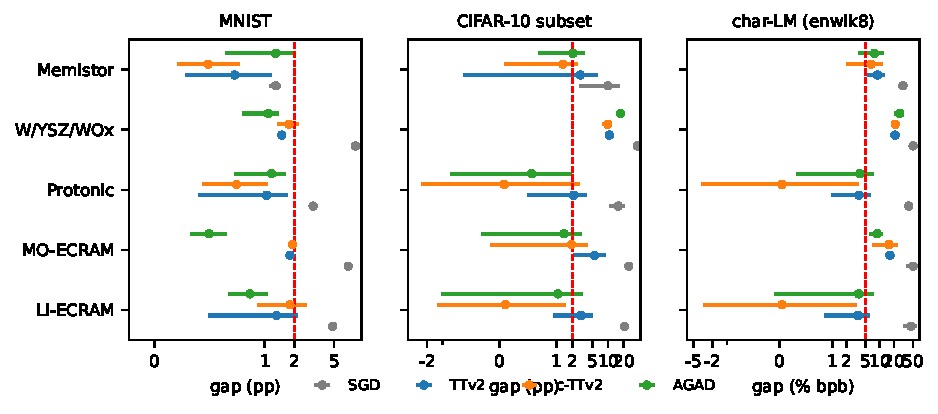
\includegraphics[width=\linewidth]{figs/fig_main}
\caption{Version 1 (superseded). Original simulator: gap to the exact-update baseline (mean and 95\% interval over 5 seeds; symmetric-log axis); the
dashed line is the gap line.}\label{fig:main}
\end{figure}

\section{Revision history and response to the independent review}\label{app:revision}
\paragraph{History.} Version 1 (October 25, 2026) reported the experiments of Appendix~\ref{app:original}. An independent
technical review (October 26, 2026) recommended major revision with thirteen findings. Version 2 answered them; the
full response, finding by finding, with the checks that confirmed or qualified each one, is \texttt{RESPONSE-TO-REVIEW.md} in
the release. The revision plan was committed before any revision run (\texttt{PLAN-REVISION.md}); its deviations R1--R\RVnDev{}
are recorded in \texttt{DEVIATIONS-PAPER.md}. Version 3 (October 26, 2026) answered a second review (eight findings;
\texttt{RESPONSE-TO-REVIEW-2.md}, plan \texttt{PLAN-REVISION-2.md}): the pulse-fidelity experiments of
Section~\ref{sec:fidelity}, the recentred fixed-symmetry control, the width contrasts paired by seed and the revised
settings tables. Version 4 (October 27, 2026) answers a third review (five findings;
\texttt{RESPONSE-TO-REVIEW-3.md}, plan \texttt{PLAN-REVISION-3.md}, committed before its runs): the per-sample stream is
compared with the literal one paired by draw, with bootstrap bounds, in a desk rerun of the update probes that keeps the
draws; the cross-cell dependence is measured by per-pair correlations that cannot cancel; the training comparison reports
both arms' labels and every rank reversal; the open training rerun of the one material cell was done; and an interval that
includes the width margin is no longer read as growth below it. Version 5 (October 27, 2026; this paper) answers a
fourth review (three findings; \texttt{RESPONSE-TO-REVIEW-4.md}, plan \texttt{PLAN-REVISION-4.md}, committed before
its runs). Version 4's five-seed rerun of the material SGD cell had joined, by seed only, two stream runs whose
initialisation and example order differed from their controls' (the random draws depend on the GPU model), and it
had put a seed-0 difference down to GPU rounding; its figures (stream gap \RYAtwoRSeqGap\,pp, change \RYAtwoRD\,pp)
are withdrawn as an unmatched, mixed-hardware diagnostic. The cell was rerun as matched triples on one GPU, and the
analysis now refuses a seed whose arms do not share both hashes. The saved pulse draws joined the deposit with a
command that rebuilds the probe tables from them, the probe table was split in two for legibility, and the abstract
states that its probe count is a point-estimate count.

\paragraph{What was repaired.}
\begin{enumerate}
\item \textbf{Random streams.} The initialisation, the data order, each tile's device population and the pulse/noise draws now
      have separate generators; every record carries the hashes of its logical initialisation and data order, and every arm
      of a seed shares them (checked). The old single stream is kept as a mode that replays the original simulator bit for bit.
\item \textbf{The reset.} The original reset moved $A$ to its symmetry point and charged 62 pulses it never applied; applied
      through the device model those pulses leave \RVresetResidPct\,\% of the displacement (from $u=0.8$ the state only reaches
      \RVresetAfter, against a symmetry point of \RVresetSp; about \RVresetPulsesHundredfold{} alternating pulses would be needed
      for a hundredfold reduction). The repaired pulse reset applies and counts every pulse; the ideal reset is reported only
      as a labelled variant.
\item \textbf{The AIHWKIT presets} are mapped one to one (shifted bounds, bound-scaled slopes, slope spread), and their pulse
      responses were compared with AIHWKIT's own (Section~\ref{sec:validation}): the mapping is \RVaihwAccepted.
\item \textbf{Measured, not assumed:} the clipping of the pulse probabilities and the lost update are recorded per layer.
\end{enumerate}
The \RVnChecks{} checks of the repairs each fail on the old behaviour or a planted fault (\RVnFaults{} faults; \RVtestsAllOk{}
on the desk and on every pod).

\paragraph{How much the repairs moved the original conclusions (diagnostic D1).} Table~\ref{tab:rev_d1} runs the original and
the repaired simulator side by side at the original selections, 3 seeds, on MNIST and a 10-epoch CIFAR slice
(\RVdOneRuns{} runs).
\begin{itemize}
\item \textbf{The random streams} moved individual cells by up to \RVdOneRngMnistMaxAbs\,pp on MNIST and
      \RVdOneRngCifarMaxAbs\,pp on CIFAR (material, i.e.\ more than 1\,pp or a label change, in \RVdOneRngMnistNMaterial{} of
      \RVdOneRngMnistN{} and \RVdOneRngCifarNMaterial{} of \RVdOneRngCifarN{} cells). With three seeds this is within the noise:
      the repaired FP-SGD alone spans \RVdOneCifarFpMin--\RVdOneCifarFpMax\,\% on the CIFAR slice. The matched controls did not
      reduce the paired-gap spread here (median \RVdOneSdRev{} against \RVdOneSdOld\,pp).
\item \textbf{The reset} moved cells by up to \RVdOneResetMnistMaxAbs\,pp on MNIST and \RVdOneResetCifarMaxAbs\,pp on CIFAR. The
      ideal reset gave no hidden advantage: a physical reset (pulse, alternating pairs or none) had an equal or smaller gap in
      \RVdOneResetBetterN{} of \RVdOneResetN{} cells.
\item \textbf{The mapping} moved Li-ECRAM by at most \RVdOneMapMnistMaxAbs\,pp on MNIST and \RVdOneMapCifarMaxAbs\,pp on CIFAR.
\item \textbf{Unchanged:} plain SGD fails by far (MNIST \RVdOneSgdMnistMin--\RVdOneSgdMnistMax\,pp, CIFAR slice
      \RVdOneSgdCifarMin--\RVdOneSgdCifarMax\,pp).
\end{itemize}

\paragraph{Wording withdrawn or narrowed.} ``Near-digital'' is not used. ``Plain SGD fails on every device'' became ``every
plain-SGD arm at the FP-selected learning rate exceeded the margin''. ``The gap does not grow with width'' became the equivalence
statement of Section~\ref{sec:scale}. ``Two device properties decide'' and ``a few hundred levels suffice'' became conditional
statements about the sweeps of Section~\ref{sec:spec}. ``The memistor lacked density, speed and energy, not accuracy'' became
``an optimistic historical-device scenario attained useful accuracy in this simulator''. ``32$\times$ today with the periphery
counted'' became the conditional projection of Section~\ref{sec:energy}. ``A bench replication'' became ``a proposed, unbuilt
bench replication protocol''. ``Every matrix is analog'' became ``the learned weight matrices use the device model; attention
products and other operations are digital''.

\begin{table*}[t]\centering\scriptsize\caption{Diagnostic D1: mean gap to FP-SGD of the same simulator (pp, 3 seeds; P/F/U against 2 pp) at the original selections. Columns: orig. = the original simulator; ideal = the repaired random streams with the original ideal reset; then the reset replaced by the pulse reset (pulse), 31 alternating pulse pairs (alt.), or none; publ. = the published-style TTv2. The AIHWKIT-mapped Li-ECRAM row uses the pulse reset for TTv2 and c-TTv2. CIFAR here is a 10-epoch slice.}\label{tab:rev_d1}
\begin{tabular}{lllcccccc}\toprule Task & Device & Alg. & orig. & ideal & pulse & alt. & none & publ.\\\midrule
MNIST & Protonic-insp. & SGD & 3.09F & 4.58U &  &  &  & \\
MNIST & Protonic-insp. & TTv2 & 1.04U & 1.60U & 0.23P & 0.66P & 1.02P & 0.99P\\
MNIST & Protonic-insp. & c-TTv2 & 0.81P & 0.62U & 0.44P & 0.97U & 1.41P & \\
MNIST & Protonic-insp. & AGAD & 1.21P & 0.99P &  &  &  & \\
MNIST & Li (old map) & SGD & 4.79F & 6.47U &  &  &  & \\
MNIST & Li (old map) & TTv2 & 1.33U & 1.19U & 0.39P & 0.36P & 0.66P & 1.43P\\
MNIST & Li (old map) & c-TTv2 & 1.51U & 0.98P & 0.80P & 0.68P & 1.00P & \\
MNIST & Li (old map) & AGAD & 0.96P & 1.00P &  &  &  & \\
MNIST & Li (AIHWKIT) & SGD &  & 6.99U &  &  &  & \\
MNIST & Li (AIHWKIT) & TTv2 &  &  & 0.40P &  &  & \\
MNIST & Li (AIHWKIT) & c-TTv2 &  &  & 0.70P &  &  & \\
MNIST & Li (AIHWKIT) & AGAD &  & 0.57P &  &  &  & \\
CIFAR-10ep & Protonic-insp. & SGD & 14.24F & 10.35F &  &  &  & \\
CIFAR-10ep & Protonic-insp. & TTv2 & 5.28U & 2.53U & 2.04U & -0.83U & -1.97U & 4.17U\\
CIFAR-10ep & Protonic-insp. & c-TTv2 & 4.59U & 3.41U & 5.97U & -0.43U & 0.65U & \\
CIFAR-10ep & Protonic-insp. & AGAD & -0.70P & -2.94U &  &  &  & \\
CIFAR-10ep & Li (old map) & SGD & 17.69F & 16.91F &  &  &  & \\
CIFAR-10ep & Li (old map) & TTv2 & 4.35F & 2.51U & 2.98U & 0.57U & 0.78U & 5.41U\\
CIFAR-10ep & Li (old map) & c-TTv2 & 6.08U & 2.27U & 1.63U & 1.48U & 0.99U & \\
CIFAR-10ep & Li (old map) & AGAD & 0.39U & -1.34U &  &  &  & \\
CIFAR-10ep & Li (AIHWKIT) & SGD &  & 17.87F &  &  &  & \\
CIFAR-10ep & Li (AIHWKIT) & TTv2 &  &  & 2.37U &  &  & \\
CIFAR-10ep & Li (AIHWKIT) & c-TTv2 &  &  & 2.71U &  &  & \\
CIFAR-10ep & Li (AIHWKIT) & AGAD &  & -1.02U &  &  &  & \\
\bottomrule\end{tabular}\end{table*}


\paragraph{Version 3's update probes (superseded).} Table~\ref{tab:v3s_rev2_probe} is version 3's analysis of the update
probes (pod sitting r6). Its sampling floor for the per-sample stream added the two methods' variances as if their draws were
independent, although the per-sample stream replays the literal stream's line firings, so the floor was too large and every
excess of the per-sample stream came out as zero. Version 4 replaces it by the paired analysis of Section~\ref{sec:fidelity}
(Table~\ref{tab:rev3_probe}). The surrogate's verdicts did not depend on this floor.

% made by revision3/analyze_rev3.py from tables/rev2_probe.tex (caption prefix and label only; do not edit)
% generated by revision2/analyze_rev2.py (do not edit)
\begin{table*}[t]\centering\scriptsize\caption{Version 3 (superseded: its sampling floor for seq treated the paired draws as independent). Update fidelity (experiment A1; Li = Li-ECRAM, MO = MO-ECRAM, Prot. = protonic-inspired): one training batch applied repeatedly from the same state by the aggregate surrogate (sur.), the per-sample stream (seq) and the literal pulse-by-pulse stream (slot). Lost = unsigned requested pulse mass removed by the probability clipping (\%); $g$ = the slot stream's realised gain along the requested update; then surrogate / seq against slot: gain difference (\%), excess relative mean difference beyond the sampling floor, median per-cell variance ratio; faithful by the pre-registered lines (gain within 10 \%, excess $\le$ 0.10, variance ratio in [0.5, 2]; for seq 5 \%, 0.05, [0.8, 1.25]).}\label{tab:v3s_rev2_probe}
\begin{tabular}{lllrrrrrl}\toprule Case & Layer & Upd. & Lost & $g$ & $\Delta g$ & excess & var.\ ratio & faithful\\\midrule
CIFAR MO AGAD & 3 (128$\times$1024) & 600 & 32.1 & 0.431 & 0.7 / -0.2 & 0.07 / 0.00 & 1.08 / 1.00 & yes / yes\\
CIFAR MO AGAD & 4 (10$\times$128) & 600 & 92.1 & 0.027 & 1.8 / 0.3 & 0.18 / 0.00 & 1.20 / 1.02 & no / yes\\
CIFAR MO AGAD & 3 (128$\times$1024) & 2000 & 15.0 & 0.700 & 1.3 / -0.0 & 0.03 / 0.00 & 1.07 / 1.00 & yes / yes\\
CIFAR MO AGAD & 4 (10$\times$128) & 2000 & 96.5 & 0.004 & 32.7 / 0.6 & 0.37 / 0.00 & 1.22 / 1.00 & no / yes\\
LM Prot. c-TTv2 & 0 (128$\times$256) & 750 & 7.6 & 0.717 & 0.3 / 0.1 & 0.01 / 0.00 & 1.00 / 1.00 & yes / yes\\
LM Prot. c-TTv2 & 9 (256$\times$128) & 750 & 0.0 & 0.972 & -1.4 / -0.5 & 0.00 / 0.00 & 0.71 / 1.01 & yes / yes\\
LM Prot. c-TTv2 & 0 (128$\times$256) & 2250 & 32.5 & 0.547 & -0.1 / 0.0 & 0.04 / 0.00 & 1.02 / 1.00 & yes / yes\\
LM Prot. c-TTv2 & 9 (256$\times$128) & 2250 & 0.0 & 0.882 & 0.2 / 0.3 & 0.00 / 0.00 & 0.73 / 1.01 & yes / yes\\
MNIST Li c-TTv2 & 0 (256$\times$784) & 1000 & 21.6 & 0.759 & 0.1 / -0.0 & 0.03 / 0.00 & 1.05 / 1.00 & yes / yes\\
MNIST Li c-TTv2 & 2 (10$\times$128) & 1000 & 3.7 & 0.990 & -0.0 / -0.0 & 0.00 / 0.00 & 1.26 / 0.98 & yes / yes\\
MNIST Li c-TTv2 & 0 (256$\times$784) & 3500 & 25.7 & 0.696 & -0.3 / -0.0 & 0.01 / 0.00 & 1.09 / 1.00 & yes / yes\\
MNIST Li c-TTv2 & 2 (10$\times$128) & 3500 & 5.0 & 0.922 & -1.1 / 0.1 & 0.00 / 0.00 & 1.55 / 1.00 & yes / yes\\
\bottomrule\end{tabular}\end{table*}


